\chapter{Deviation from the Mean}\label{deviation_chap}

%\section{Why the Mean?}

In the previous chapter, we took it for granted that expectation is
useful and developed a bunch of techniques for calculating
\idx{expected value}s.  But why should we care about this value?
After all, a random variable may never take a value anywhere near its
expectation.

The most important reason to care about the mean value comes from its
connection to estimation by sampling.  For example, suppose we want to
estimate the average age, income, family size, or other measure of a
population.  To do this, we determine a random process for selecting
people---say, throwing darts at census lists.  This process makes the
selected person's age, income, and so on into a random variable whose
\emph{mean} equals the \emph{actual \idx{average}} age or income of
the population.  So, we can select a random sample of people and
calculate the average of people in the sample to estimate the true
average in the whole population.  But when we make an estimate by
repeated sampling, we need to know how much confidence we should have
that our estimate is OK, and how large a sample is needed to reach a
given confidence level.  The issue is fundamental to all experimental
science.  Because of random errors---\emph{noise}---repeated
measurements of the same quantity rarely come out exactly the same.
Determining how much confidence to put in experimental measurements is
a fundamental and universal scientific issue.  Technically, judging
sampling or measurement accuracy reduces to finding the probability
that an estimate \emph{deviates} by a given amount from its expected
value.

Another aspect of this issue comes up in engineering.  When designing
a sea wall, you need to know how strong to make it to withstand
tsunamis for, say, at least a century.  If you're assembling a
computer network, you might need to know how many component failures it
should tolerate to likely operate without maintenance for at
least a month.  If your business is insurance, you need to know how
large a financial reserve to maintain to be nearly certain of paying
benefits for, say, the next three decades.  Technically, such
questions come down to finding the probability of \emph{extreme}
deviations from the mean.

This issue of \term{deviation from the mean} is the focus of this
chapter.

\begin{editingnotes}
A random variable may never take a value anywhere near its expected value,
so why is its expected value important?  The reason is suggested by a
property of gambling games that most people recognize intuitively.
Suppose your gamble hinges on the roll of two dice, where you win if the
sum of the dice is seven.  If the dice are fair, the probabilty you win is
$1/6$, which is also your expected number of wins in one roll.  Of course
there's no such thing as $1/6$ of a win in one roll, since either you win
or you don't.  But if you play \emph{many times}, you would expect that
the \emph{fraction} of times you win would be close to $1/6$.  In fact, if
you played a lot of times and found that your fraction of wins wasn't
pretty close to $1/6$, you would become pretty sure that the dice weren't
fair.
\end{editingnotes}

\section{Markov's Theorem}

\begin{editingnotes}

The first result is Markov's Theorem, which gives a simple, but typically
coarse, upper bound on the probability that the value of a random variable
is more than a certain multiple of its mean.  Markov's result holds if we
know nothing about a random variable except what its mean is and that its
values are nonnegative.  Accordingly, Markov's Theorem is very general,
but also is much weaker than results which take into account more
information about the distribution of the variable.

In many situations, we not only know the mean, but also another numerical
quantity called the \emph{variance} of the random variable.  The second
basic result is Chebyshev's Theorem, which combines Markov's Theorem and
information about the variance to give more refined bounds.

\end{editingnotes}

Markov's theorem gives a generally coarse estimate of the probability
that a random variable takes a value \emph{much larger} than its mean.
It is an almost trivial result by itself, but it actually leads fairly
directly to much stronger results.

The idea behind \idx{Markov's Theorem} can be explained by considering
the quantity known as \emph{intelligence quotient}, \idx{\IQ}, which
remains in wide use despite doubts about its legitimacy.  \IQ\ was
devised so that its average measurement would be 100.  This
immediately implies that at most 1/3 of the population can have an
\IQ\ of 300 or more, because if more than a third had an \IQ\ of 300,
then the average would have to be \emph{more} than $(1/3)\cdot 300 =
100$.  So, the probability that a randomly chosen person has an
\IQ\ of 300 or more is at most 1/3.  By the same logic, we can also
conclude that at most 2/3 of the population can have an \IQ\ of 150 or
more.

Of course, these are not very strong conclusions.  No \IQ\ of over 300
has ever been recorded; and while many \IQ's of over 150 have been
recorded, the fraction of the population that actually has an
\IQ\ that high is very much smaller than 2/3.  But though these
conclusions are weak, we reached them using just the fact that the
average \IQ\ is 100---along with another fact we took for granted,
that \IQ\ is never negative.  Using only these facts, we can't
derive smaller fractions, because there are nonnegative random
variables with mean 100 that achieve these fractions.  For example, if
we choose a random variable equal to 300 with probability 1/3 and 0
with probability 2/3, then its mean is 100, and the probability of a
value of 300 or more really is 1/3.  \begin{editingnotes}
But we'll get real mileage out of
this coarse bound in later sections.
\end{editingnotes}

\begin{editingnotes}

Note that very different distributions can still have the same mean.

\begin{example}
  Suppose that we roll a fair die.  This gives a random variable
  uniformly distributed on $1, 2, \dots 6$.  The mean, or expected
  value, is 3.5.  Of course, this random variable never takes on
  exactly the expected value; in fact, the outcome deviates from the
  mean by at least 0.5 with probability 1.  Furthermore, there is a
  $\frac{2}{3}$ probability that the outcome deviates from the mean by
  at least 1.5 (roll 1, 2, 5, or 6), a $\frac{1}{3}$ probability that
  the outcome deviates by at least 2.5 (roll 1 or 6), and zero
  probability that the outcome deviates by more than 2.5.
\end{example}

\begin{example}
  A random variable with the binomial distribution is much less likely
  to deviate far from the mean.  For example, suppose we flip 100
  fair, mutually independent coins and count the number of heads.  The
  expected number of heads is 50.  There is an 8\% chance that the
  outcome is exactly the mean, and the probability of flipping more
  than 75 heads or fewer than 25 is less than 1 in a billion.
\end{example}

The probability distribution functions for the two preceding examples
are graphed in Figure~\ref{fig:uniform} and Figure~\ref{fig:binom2}.
There is a big difference!  For the uniform distribution, the graph is
flat; that is, outcomes far from the mean are as likely as outcomes
close to the mean.  However, the binomial distribution has a peak
centered on the expected value and the tails fall off rapidly.  This
shape implies that outcomes close to the expected value are vastly
more likely than outcomes far from the expected value.  In other
words, a random variable with the binomial distribution rarely
deviates far from the mean.
\begin{figure}
  \centerline{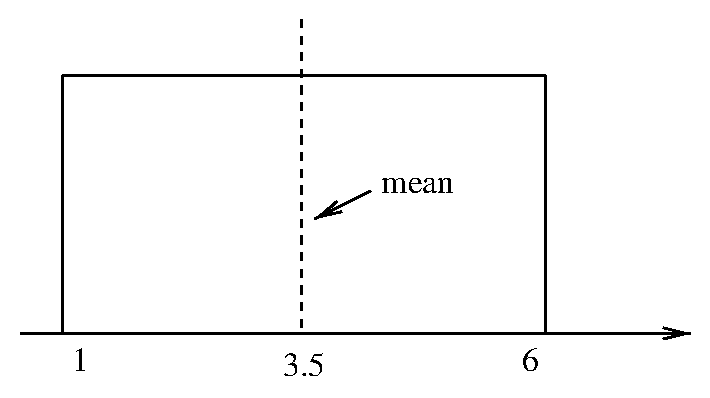
\includegraphics[height=2in]{uniform}}
  \caption{This is a graph of the uniform distribution arising from
    rolling a fair die.  Outcomes within the range of the distribution
    are equally likely, regardless of distance from the mean.}
  \label{fig:uniform}
\end{figure}
\begin{figure}
  \centerline{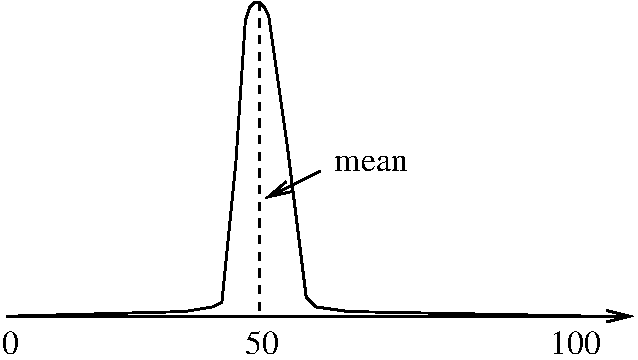
\includegraphics[height=2in]{binom2}}
  \caption{This is a rough graph of the binomial distribution given by
    the number of heads that come up when we flip 100 fair, mutually
    independent coins.  Outcomes close to the mean are much more
    likely than outcomes far from the mean.}
  \label{fig:binom2}
\end{figure}

On the other hand, we can define a random variable that always
deviates substantially from its expected value.  Suppose that we glue
100 coins together, so that with probability 1/2 all are heads and
with probability 1/2 all are tails.  The graph of the probability
distribution function for the number of heads is shown in
Figure~\ref{fig:nasty}.  While the expected value of this random
variable is 50, the actual value is always 0 or~100.
\begin{figure}
  \centerline{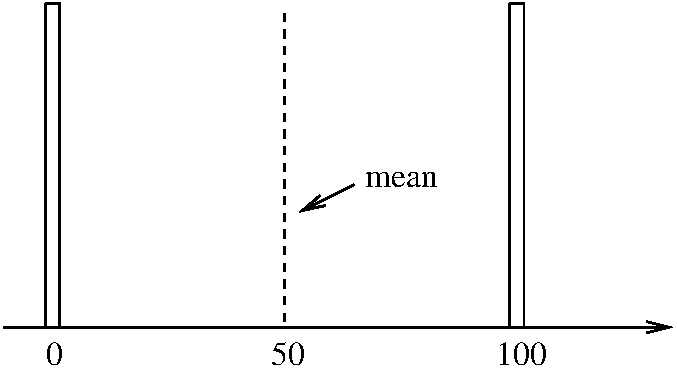
\includegraphics[height=2in]{nasty}}
  \caption{This is the nasty distribution corresponding to the number
    of heads that come up when we flip 100 coins that are all glued
    together. The outcome always differs from the mean by at
    least~50.}
  \label{fig:nasty}
\end{figure}

Even in this last example, however, the random variable is twice the
mean with probability only $1/2$.  In fact, we will see that this is a
worst-case distribution with respect to deviation from the mean.

\subsection*{Theorem Statement and Some Applications}

\end{editingnotes}

\begin{theorem}[\idx{Markov's Theorem}]\label{markovthm}
  If R is a nonnegative random variable, then for all $x > 0$
\begin{equation}\label{markovx}
    \pr{R \geq x} \leq \frac{\expect{R}}{x}.
\end{equation}
\end{theorem}

\begin{editingnotes}

Before we prove Markov's Theorem, let's apply it to the three examples in
the preceding subsection.  First, let the random variable~$R$ be the
number that comes up when we roll a fair die.  By Markov's Theorem, the
probability of rolling a 6 is at most:
\[
\pr{R \geq 6} \leq \frac{\expect{R}}{6} = \frac{3.5}{6} = 0.583\dots
\]
This conclusion is true, but weak.  The actual probability of rolling
a 6 is $1/6 = 0.166\dots$.

This is typical of Markov's Theorem.  The theorem is easy to apply
because it requires so little information about a random variable,
only the expected value and nonnegativity.  But as a consequence,
Markov's Theorem often leads to weak conclusions like the one above.

Suppose that we flip 100 mutually independent, fair coins.  Markov's
Theorem says that the probability of throwing 75 or more heads is at
most:
\[
\pr{\text{heads} \geq 75} \leq \frac{\expect{\text{heads}}}{75} =
\frac{50}{75} = \frac{2}{3}.
\]
Markov's Theorem says that the probability of 75 or more heads is at
most $2/3$, but the actual probability is less than 1 in a
billion!

These two examples show that Markov's Theorem gives weak results for
well-behaved random variables; however, the theorem is actually right
for some examples.  Suppose we flip 100 fair coins and use Markov's
Theorem to compute the probability of getting all heads:
\[
\pr{\text{heads} \geq 100} \leq \frac{\expect{\text{heads}}}{100} =
\frac{50}{100} = \frac{1}{2}.
\]
If the coins are mutually independent, then the actual probability of
getting all heads is a miniscule 1 in $2^{100}$.  In this case, Markov's
Theorem looks very weak.  However, in applying Markov's Theorem, we made
no independence assumptions.  In fact, if all the coins are glued
together, then probability of throwing all heads is exactly $1/2$.
In this nasty case, Markov's Theorem is actually tight!

\subsection{Proof of Markov's Theorem}

Let~$R$ be the weight of a person selected randomly and uniformly.
Suppose that an average person weighs 100 pounds; that is, $\expect{R} =
100$.  What is the probability that a random person weighs at least
200 pounds?

There is insufficient information for an exact answer.  However, we
can safely say that the probability that $R \geq 200$ is most
$1/2$.  If more than half of the people weigh 200 pounds or
more, then the average weight would exceed 100 pounds, even if
everyone else weighed zero!  Markov's Theorem gives the same result:
\begin{displaymath}
  \pr{R \geq 200} \leq \frac{\expect{R}}{200} = \frac{100}{200} = \frac{1}{2}.
\end{displaymath}

Reasoning similar to that above underlies the proof of Markov's
Theorem.  Since expectation is a weighted average of all the outcomes
of the random variable, that is, a sum over all the variables the random
variable can assume, we can give a lower bound on the expectation by
removing some of the terms from the sum defining the expectation; this
new sum can then be modified into an expression involving the
probability of an event in the tail $[R \geq x]$.

\end{editingnotes}

\begin{proof}%[Proof of Markov's Theorem]

\iffalse
\begin{align}
  \expect{R}
  & = \expcond{R}{R < x}\pr{R<x} + \expcond{R}{R \geq x}\pr{R \geq x}
       & \text{(total expectation)}\notag\\
  & \geq \expcond{R}{R \geq x}\pr{R \geq x}
       & \text{(because $R \geq 0$)}\notag\\
  & \geq x \pr{R \geq x}.\label{markovproof}
\end{align}

Let $y$ vary over the range of~$R$.  Then for any $x > 0$
\begin{align}
  \expect{R}
  & \eqdef \sum_{y} y\pr{R=y}\notag\\
  & \geq \sum_{y \geq x} y\pr{R=y} & \text{(because $R \geq 0$)}\notag\\
  & \geq \sum_{y \geq x} x\pr{R=y}\notag\\
  & = x \sum_{y \geq x} \pr{R=y}\notag\\
  & = x \pr{R \geq x}.\label{markovproof}
\end{align}

\begin{align}
  \expect{R}
   & \eqdef \sum_{y} y\pr{R=y}\notag\\
   & \geq \sum_{y \geq x} y\pr{R=y}
     \geq \sum_{y \geq x} x\pr{R=y}
      = x \sum_{y \geq x} \pr{R=y}\notag\\
  & = x \pr{R \geq x},\label{markovproof}
\end{align}
where the first inequality follows from the fact that $R \geq 0$.
\fi

Let $I_x$ be the indicator variable for the event $[R \geq x]$.  Then
\[
xI_x \leq R
\]
holds for all values of $R$ since $R \geq 0$.  Taking expectations of
both sides yields
\[
x \pr{R \geq x}    \iffalse  = \expect{xI_x} \fi
\leq \expect{R},
\]
and then dividing both sides of this inequality by $x$
gives~\eqref{markovx}.
\end{proof}

\iffalse
We will show that $\expect{R} \geq x \pr{R \geq x}$.  Dividing
both sides by $x$ gives the desired result.

So let $I_x$ be the indicator variable for the event $[R \geq x]$, and
consider the random variable $x I_x$.  Note that
\[
R \geq x I_x,
\]
because at any sample point $\omega$,
\begin{itemize}
\item if $R(\omega) \geq x$ then $R(\omega) \geq x = x\cdot 1 = x I_x(\omega)$, and
\item if $R(\omega) < x$ then $R(\omega) \geq 0 = x \cdot 0 = xI_x(\omega)$.
\end{itemize}
Therefore,
\begin{align*}
\expect{R} & \geq \expect{x I_x} & (\text{since } R \geq xI_x)\\
   & = x \expect{I_x} & \text{(linearity of $\expect{\cdot}$)}\\
   & = x \pr{I_x=1}  &  \text{($I_x$ is an indicator)}\\
   & = x \pr{R \geq x}.  &  (\text{def\ of $I_x$})
\end{align*}

\fi

Our focus is deviation from the mean, so it's useful to rephrase
Markov's Theorem this way:
\begin{corollary}
If $R$ is a nonnegative random variable, then for all $c \geq 1$
\begin{equation}
\pr{R \geq c \cdot \expect{R}\ }  \leq  \frac{1}{c}.\label{markovaboveemean}
\end{equation}
\end{corollary}
This Corollary follows immediately from Markov's Theorem\eqref{markovthm}
by letting $x$ be $c \cdot \expect{R}$.

\iffalse
This gives:
\[
\pr{R \geq c \cdot \expect{R}\ } \leq \frac{\expect{R}}{c \cdot \expect{R}} =
\frac{1}{c}.
\]
\end{proof}
\fi

\subsection{Applying Markov's Theorem}

Let's go back to the \idx{Hat-Check problem} of
Section~\ref{sec:hat_check}.  Now we ask what the probability is that
$x$ or more men get the right hat, this is, what the value of $\pr{G
  \geq x}$ is.

We can compute an upper bound with Markov's Theorem.  Since we know
$\expect{G}=1$, Markov's Theorem implies
\[
\pr{G \geq x} \leq \frac{\expect{G}}{x} = \frac{1}{x}.
\]
For example, there is no better than a 20\% chance that 5 men get the
right hat, regardless of the number of people at the dinner party.

The \idx{Chinese Appetizer problem} is similar to the Hat-Check
problem.  In this case, $n$ people are eating different appetizers
arranged on a circular, rotating Chinese banquet tray.  Someone then
spins the tray so that each person receives a random appetizer.  What
is the probability that everyone gets the same appetizer as before?

There are $n$ equally likely orientations for the tray after it stops
spinning.  Everyone gets the right appetizer in just one of these $n$
orientations.  Therefore, the correct answer is $1/n$.

But what probability do we get from Markov's Theorem?  Let the random
variable~$R$ be the number of people that get the right appetizer.  
%We showed in previous notes that $\expect{R} = 1$.  
Then of course $\expect{R} = 1$, so
applying Markov's Theorem, we find:
\begin{displaymath}
  \pr{R \geq n} \leq \frac{\expect{R}}{n} = \frac{1}{n}\,.
\end{displaymath}
So for the Chinese appetizer problem, Markov's Theorem is precisely
right!

Unfortunately, Markov's Theorem is not always so accurate.  For
example, it gives the same $1/n$ upper limit for the probability that
everyone gets their own hat back in the Hat-Check problem, where the
probability is actually $1/(n!)$.  So for Hat-Check, Markov's Theorem
gives a probability bound that is way too large.

\subsection{Markov's Theorem for Bounded Variables}

Suppose we learn that the average \IQ\ among MIT students is 150 (which is
not true, by the way).  What can we say about the probability that an MIT
student has an \IQ\ of more than 200?  Markov's theorem immediately tells
us that no more than $150/200$ or $3/4$ of the students can have such a
high \IQ.  Here, we simply applied Markov's Theorem to the random variable
$R$ equal to the \IQ\ of a random MIT student to conclude:
\[
\pr{R > 200} \leq \frac{\expect{R}}{200}= \frac{150}{200} = \frac{3}{4}.
\]

But let's observe an additional fact (which may be true): no MIT student
has an \IQ\ less than 100.  This means that if we let $T \eqdef R-100$,
then $T$ is nonnegative and $\expect{T} = 50$, so we can apply Markov's
Theorem to $T$ and conclude:
\[
\pr{R > 200} = \pr{T > 100} \leq \frac{\expect{T}}{100}= \frac{50}{100} =
\frac{1}{2}.
\]
So only half, not 3/4, of the students can be as amazing as they think
they are.  A bit of a relief!

In fact, we can get better bounds applying Markov's Theorem to $R-b$
instead of $R$ for any lower bound $b$ on $R$ (see
Problem~\ref{PS_Markov_with_bounded_RVs}).  Similarly, if we have any
upper bound $u$ on a random variable $S$, then $u-S$ will be a
nonnegative random variable, and applying Markov's Theorem to $u-S$
will allow us to bound the probability that $S$ is much \emph{less}
than its expectation.

\iffalse
Suppose we know that $R \geq \ell$, then can we do better?
Let $T=R-\ell$.  Note that $T \geq 0$.  So, we can use Markov's
Theorem on $T$, to say that 
\begin{eqnarray*}
\pr{R  \geq x }   & = &   \pr{T \geq x -\ell} 
  \leq 
  \frac{\expect{T}}{x -\ell} 
  =   \frac{\expect{R - \ell}}{x - \ell}
  =   \frac{\expect{R} - \ell}{x - \ell} \\
  %& < &  \frac{\expect{R}}{x}
\end{eqnarray*}
%$\pr{R - \ell \geq x} = \pr{T \geq x} 
%\leq 
%\frac{\expect{T}}{x} 
%= \frac{\expect{R - \ell}}{x} =
%= \frac{\expect{R}{x} - \ell/x$
This gives a somewhat better bound on the probability that
$R$ goes crazy!  
\fi

\begin{editingnotes}

\subsection{Why \emph{R} Must be Nonnegative}

Remember that Markov's Theorem applies only to nonnegative random
variables!  The following example shows that the theorem is false if this
restriction is removed.  Let $R$ be -10 with probability $1/2$ and 10 with
probability $1/2$.  Then we have:
\[
\expect{R} = -10 \cdot \frac{1}{2} + 10 \cdot \frac{1}{2} = 0
\]
Suppose that we now tried to compute $\pr{R \geq 5}$ using Markov's
Theorem:
\begin{displaymath}
  \pr{R \geq 5} \leq \frac{\expect{R}}{5} = \frac{0}{5} = 0.
\end{displaymath}
This is the wrong answer: $R$ is at least 5 with
probability $1/2$!

On the other hand, we can still apply Markov's Theorem indirectly to
derive a bound on the probability that an arbitrary variable like $R$ is 5
more.  Namely, given any random variable $R$ with expectation 0 and
values $\geq -10$, we can conclude that $\pr{R \geq 5} \le 2/3$.
\begin{proof}
Let $T \eqdef R+10$.  Now $T$ is a nonnegative random variable with
expectation $\expect{R + 10} = \expect{R}+10= 10$, so Markov's Theorem
applies and tells us that $\pr{T \geq 15} \le 10/15 = 2/3$.  But $T \geq
15$ iff $R \geq 5$, so $\pr{R \geq 5} \leq 2/3$, as claimed.
\end{proof}

\subsection{Deviation Below the Mean}

Markov's Theorem says that a random variable is unlikely to greatly exceed
the mean.  Correspondingly, there is a theorem that says a random variable
is unlikely to be much smaller than its mean.

\begin{theorem}
\label{th:below}
Let $l$ be a real number and let $R$ be a random variable such that $R
\leq l$.  For all $x < l$, we have:
\[
\pr{R \leq x} \leq \frac{l - \expect{R}}{l - x}.
\]
\end{theorem}

\begin{proof}
The event that $R \leq x$ is the same as the event that $l - R \geq l -
x$.  Therefore:
\begin{align}
\pr{R \leq x} &  = \pr{l - R \geq l - x}\notag\\
 & \leq \frac{\expect{l - R}}{l - x}. & \text{(Markov' Theorem)}\label{LR}
\end{align}
Applying Markov's Theorem in line~\eqref{LR} is permissible
since $l - R$ is a nonnegative random variable and $l - x > 0$.
\end{proof}

For example, suppose that the class average on the 6.042 midterm was
75/100.  What fraction of the class scored below 50?

There is not enough information here to answer the question exactly,
but Theorem~\ref{th:below} gives an upper bound.  Let $R$ be the score
of a random student.  Since 100 is the highest possible score, we
can set $L = 100$ to meet the condition in the theorem that $R \leq
L$.  Applying Theorem~\ref{th:below}, we find:
\begin{displaymath}
  \pr{R \leq 50} \leq \frac{100 - 75}{100 - 50} = \frac{1}{2}\,.
\end{displaymath}

That is, at most half of the class scored 50 or worse.  This makes
sense; if more than half of the class scored 50 or worse, then the
class average could not be 75, even if everyone else scored 100.
As with Markov's Theorem, Theorem~\ref{th:below} often gives weak
results.  In fact, based on the data given, the entire class could
have scored above 50.

\subsubsection*{Using Markov To Analyze Non-Random Events}

In the previous examples, we used a theorem about a random variable to
conclude facts about non-random data.  For example, we concluded that
if the average score on a test is 75, then at most $1/2$ the
class scored 50 or worse.  There is no randomness in this problem,
so how can we apply Theorem~\ref{th:below} to reach this conclusion?

The explanation is not difficult.  For any set of scores $S = \set{s_1,
s_2, \dots, s_n}$, we introduce a random variable $R$ such that
\[
\pr{R = s_i} = \frac{\text{(\# of students with score $s_i$)}}{n}
\]
We then use Theorem~\ref{th:below} to conclude that $\pr{R \leq 50}
\leq 1/2$.  To see why this means (with certainty) that at most
$1/2$ of the students scored 50 or less, we observe that
\begin{eqnarray*}
\pr{R \leq 50}  & = & \sum_{s_i \leq 50} \pr{R = s_i} \\
  & = & \sum_{s_i \leq 50} \frac{\text{(\# of students with score $s_i$)}}{n} \\
  & = & \frac{1}{n} \text{(\# of students with score 50 or less)}.
\end{eqnarray*}
So, if $\pr{R \leq 50} \leq 1/2$, then the number of students
with score 50 or less is at most $n/2$.

\end{editingnotes}

\begin{problems}

\practiceproblems
\pinput{TP_above_average_fingers}

\classproblems
\pinput{CP_cold_cows_markov}

\homeworkproblems
\pinput{PS_Markov_with_bounded_RVs}

\examproblems
\pinput{FP_hot_cows_markov}

\end{problems}

\section{Chebyshev's Theorem}

We've seen that Markov's Theorem can give a better bound when applied
to $R-b$ rather than $R$.  More generally, a good trick for getting
stronger bounds on a random variable $R$ out of Markov's Theorem is to
apply the theorem to some cleverly chosen function of $R$.  Choosing
functions that are powers of the absolute value of $R$ turns out to be
especially useful.  In particular, since $\abs{R}^z$ is nonnegative
for any real number $z$, Markov's inequality also applies to the event
$[\, \abs{R}^z \geq x^z]$.  But for positive $x,z>0$ this event is equivalent
to the event $[\, \abs{R} \geq x]$ for , so we have:

\iffalse
It is a bit messy to apply Markov's Theorem directly to this problem,
because it's generally not easy to compute $\expect{\ \abs{R -
\expect{R}}\ }$.  However, since $\abs{R}$ and hence $\abs{R}^k$ are
nonnegative variables for any $R$, Markov's inequality also applies to the
event $[\abs{R}^k \geq x^k]$.  But this event is equivalent to the event
$[\abs{R} \geq x]$, so we have:
\fi

\begin{lemma}\label{lem:Markov2}
For any random variable~$R$ and positive real numbers $x,z$,
\[
\pr{\abs{R} \geq x} \leq \frac{\expect{\strut \abs{R}^z}}{x^z}.
\]
\end{lemma}
Rephrasing~\eqref{lem:Markov2} in terms of $\abs{R - \expect{R}\, }$,
the random variable that measures $R$'s deviation from its mean, we
get

\begin{equation}\label{chebE2}
  \prob{\,\abs{R - \expect{R}\,} \geq x} \leq \frac{\expect{(\abs{R -
        \expect{R}})^z}}{x^z}.
\end{equation}
When $z$ is positive and even, $(R - \expect{R})^z$ is nonnegative, so
the absolute value on the right-hand side of the
inequality~\eqref{chebE2} is redundant.  The case when $z =2$ turns
out to be so important that the numerator of the right-hand side has
been given a name:

\begin{definition}\label{defvar}
The \term{variance} of a random variable $R$ is:
\[
\variance{R} \eqdef \Expect{(R - \expect{R})^2}.
\]
\end{definition}
Variance is also known as \term{mean square deviation}.

The restatement of~\eqref{chebE2} for $z=2$ is known as
\term{Chebyshev's Theorem}.\footnote{There are Chebyshev Theorems in
  several other disciplines, but Theorem~\ref{chebthm} is the only one
  we'll refer to.}
\begin{theorem}[Chebyshev]\label{chebthm}
  Let $R$ be a random variable and $x \in \reals^+$.  Then
\[
\prob{\abs{R - \expect{R}\, } \geq x} \leq \frac{\variance{R}}{x^2}.
\]
\end{theorem}

The expression $\expect{(R - \expect{R})^2}$ for variance is a bit
cryptic; the best approach is to work through it from the inside out.  The
innermost expression $R - \expect{R}$ is precisely the deviation of $R$
above its mean.  Squaring this, we obtain $(R - \expect{R})^2$.  This is
a random variable that is near 0 when $R$ is close to the mean and is a
large positive number when $R$ deviates far above or below the mean.  So
if $R$ is always close to the mean, then the variance will be small.  If
$R$ is often far from the mean, then the variance will be large.

\subsection{Variance in Two Gambling Games}

The relevance of variance is apparent when we compare the following
two gambling games.

\textbf{Game A:} We win \$2 with probability $2/3$ and lose \$1 with probability
$1/3$.

\textbf{Game B:} We win \$1002 with probability $2/3$ and lose \$2001 with
probability $1/3$.

Which game is better financially?  We have the same probability, 2/3,
of winning each game, but that does not tell the whole story.  What about
the expected return for each game?  Let random variables $A$ and $B$ be
the payoffs for the two games.  For example, $A$ is 2 with probability
2/3 and -1 with probability 1/3.  We can compute the
expected payoff for each game as follows:
\begin{eqnarray*}
\expect{A} = 2 \cdot \frac{2}{3} + (-1) \cdot \frac{1}{3} = 1, \\
\expect{B} = 1002 \cdot \frac{2}{3} + (-2001) \cdot \frac{1}{3} = 1.
\end{eqnarray*}

The expected payoff is the same for both games, but the games are very
different.  This difference is not apparent in their expected value,
but is captured by variance.  We can compute the $\variance{A}$ by
working ``from the inside out'' as follows:
\begin{eqnarray*}
A - \expect{A}
        & = &   \left\{
                \begin{array}{cl}
                        1 & \text{ with probability } \frac{2}{3} \\
                        -2 & \text{ with probability } \frac{1}{3}
                \end{array}
                \right. \\
(A - \expect{A})^2
        & = &   \left\{
                \begin{array}{cl}
                        1 & \text{ with probability } \frac{2}{3} \\
                        4 & \text{ with probability } \frac{1}{3}
                \end{array}
                \right. \\
\expect{(A - \expect{A})^2}
        & = &   1 \cdot \frac{2}{3} + 4 \cdot \frac{1}{3} \\
\variance{A} & = & 2.
\end{eqnarray*}

Similarly, we have for $\variance{B}$:
\begin{eqnarray*}
B - \expect{B}
        & = &   \left\{
                \begin{array}{cl}
                        1001 & \text{ with probability } \frac{2}{3} \\
                        -2002 & \text{ with probability } \frac{1}{3}
                \end{array}
                \right. \\
(B - \expect{B})^2
        & = &   \left\{
                \begin{array}{cl}
                        1,002,001 & \text{ with probability } \frac{2}{3} \\
                        4,008,004 & \text{ with probability } \frac{1}{3}
                \end{array}
                \right. \\
\expect{(B - \expect{B})^2}
        & = &   1,002,001 \cdot \frac{2}{3} + 4,008,004 \cdot \frac{1}{3} \\
\variance{B} & = & 2,004,002.
\end{eqnarray*}

The variance of Game A is 2 and the variance of Game B is more than
two million!  Intuitively, this means that the payoff in Game A is
usually close to the expected value of \$1, but the payoff in Game B
can deviate very far from this expected value.

High variance is often associated with high risk.  For example, in ten
rounds of Game A, we expect to make \$10, but could conceivably lose
\$10  instead.  On the other hand, in ten rounds of game B, we also
expect to make \$10, but could actually lose more than \$20,000!

\subsection{Standard Deviation}

In Game B above, the deviation from the mean is 1001 in one outcome
and -2002 in the other.  But the variance is a whopping 2,004,002.
The happens because the ``units'' of variance are wrong: if the random
variable is in dollars, then the expectation is also in dollars, but
the variance is in square dollars.  For this reason, people often
describe random variables using \emph{standard deviation} instead of
variance.

\begin{definition}
The \term{standard deviation} $\sigma_R$ of a random variable $R$ is
the square root of the variance:
\[
\sigma_R \eqdef \sqrt{\variance{R}} = \sqrt{\expect{(R - \expect{R})^2}}.
\]      
\end{definition}

So the standard deviation is the square root of the mean square
deviation, or the \term{root mean square} for short.  It has the same
units---dollars in our example---as the original random variable and
as the mean.  Intuitively, it measures the average deviation from the
mean, since we can think of the square root on the outside as
canceling the square on the inside.

\begin{example}
The standard deviation of the payoff in Game B is:
\[
    \sigma_B  = \sqrt{\variance{B}} = \sqrt{2,004,002} \approx 1416.
\]

The random variable~$B$ actually deviates from the mean by either
positive 1001 or negative 2002, so the standard deviation of 1416
describes this situation more closely than the value in the millions
of the variance.
\end{example}

For bell-shaped distributions like the one illustrated in
Figure~\ref{fig:stdev}, the standard deviation measures the ``width''
of the interval in which values are most likely to fall.
\begin{figure}
  \centerline{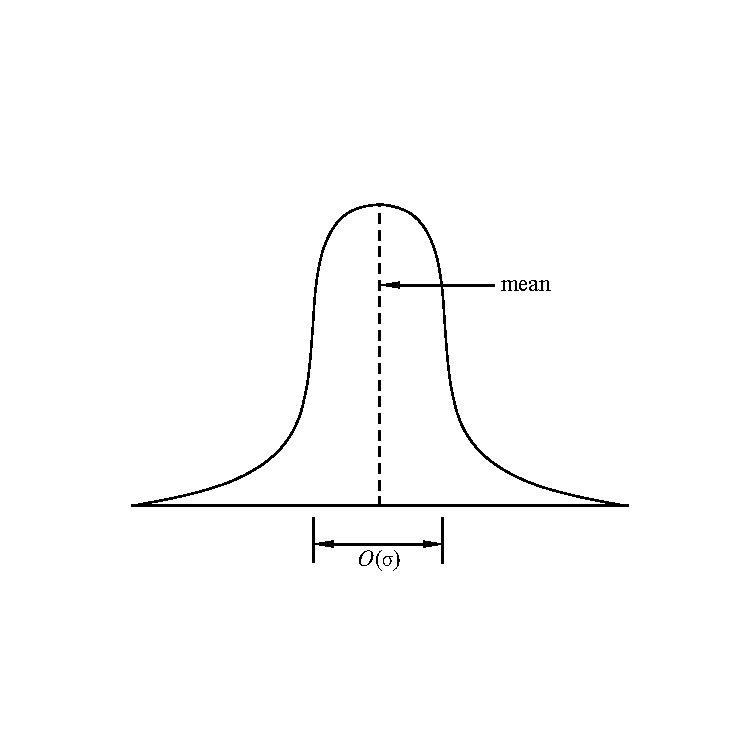
\includegraphics[height=2in]{stdev}}
  \caption{The standard deviation of a distribution indicates how wide the
    ``main part'' of it is.}
  \label{fig:stdev}
\end{figure}
This can be more clearly explained by rephrasing Chebyshev's Theorem
in terms of standard deviation, which we can do by substituting $x = c
\sigma_R$ in~\eqref{markovx}:
\begin{corollary}\label{cor:cheby}
Let $R$ be a random variable, and let $c$ be a positive real number.
\begin{equation}\label{markovcexp}
\prob{\abs{R - \expect{R}} \geq c \sigma_R} \leq \frac{1}{c^2}.
\end{equation}
\end{corollary}
Now we see explicitly how the ``likely'' values of $R$ are clustered
in an $O(\sigma_R)$-sized region around $\expect{R}$, confirming that
the standard deviation measures how spread out the distribution of $R$
is around its mean.

\iffalse
\begin{proof}
  Substituting $x = c \sigma_R$ in~\eqref{markovx} gives:
  \begin{displaymath}
    \prob{\card{R - \expect{R}} \geq c \sigma_R}
    \leq
    \frac{\variance{R}}{(c \sigma_R)^2}
    =  \frac{\sigma_R^2}{(c \sigma_R)^2}
    = \frac{1}{c^2}.
  \end{displaymath}

%  The last equality holds because variance is the square of standard
% deviation: $\variance{R} = \sigma_R^2$.

\end{proof}

\fi

\subsubsection{The IQ\ Example}\label{IQsec}

The standard \idx{standard deviation} of \IQ's regularly turns out to
be about 15 even across different populations.  This additional fact
along with the national average \idx{\IQ}\ being 100 allows a better
determination of the occurrence of \IQ's of 300 or more.

Let the random variable $R$ be the \IQ\ of a random person.  So
$\expect{R} = 100$, $\sigma_R = 15$ and $R$ is nonnegative.  We want
to compute $\prob{R \geq 300}$.

We have already seen that Markov's Theorem~\ref{markovthm} gives a coarse
bound, namely,
\[
  \prob{R \geq 300} \leq \frac{1}{3}.
\]
Now we apply Chebyshev's Theorem to the same problem:
\[
\prob{R \geq 300} = \prob{\abs{R - 100} \geq 200} \leq
\frac{\variance{R}}{200^2} = \frac{15^2}{200^2} \approx \frac{1}{178}.
\]
\iffalse
The purpose of the first step is to express the desired probability in the
form required by Chebyshev's Theorem; the equality holds because $R$ is
nonnegative.  Chebyshev's Theorem then yields the inequality.\fi

So Chebyshev's Theorem implies that at most one person in 178
has an \IQ\ of 300 or more.  We have gotten a much tighter bound using
additional information---the variance of $R$---than we could get
knowing only the expectation.

\begin{problems}
\examproblems
\pinput{FP_hot_cows_chebyshevS15}
\end{problems}

\section{Properties of Variance}\label{variance_sec}
Variance is the average \emph{of the square} of the distance from the
mean.  For this reason, variance is sometimes called the ``mean square
deviation.''  Then we take its square root to get the standard
deviation---which in turn is called ``root mean square deviation.''

But why bother squaring?  Why not study the actual distance from the
mean, namely, the absolute value of $R - \expect{R}$, instead of its
root mean square?  The answer is that variance and standard
deviation have useful properties that make them much more important in
probability theory than average absolute deviation.  In this section,
we'll describe some of those properties.  In the next section, we'll
see why these properties are important.

\iffalse
Focus on the variance and standard deviation of $R$ may seem a little
unexpected.  After all, these definitions arose from asking about the
probability that the absolute deviation $\abs{R - \expect{R}}$ was
large.  To get a better grip on the probability of deviation, we
squared it to get the Chebyshev Bound, this led us to the convoluted
concept of root mean square deviation.
\fi

\begin{editingnotes}
The problem with this definition is that the positive and negative
deviations from the mean exactly cancel.  By linearity of expectation,
we have:
\[
  \expect{R - \expect{R}} = \expect{R} - \expect{\expect{R}}.
\]
Since $\expect{R}$ is a constant, its expected value is itself. Therefore
\[
\expect{R - \expect{R}} = \expect{R} - \expect{R} = 0.
\]
By this definition, every random variable has zero variance.  That is not
useful!  Because of the square in the conventional definition, both
positive and negative deviations from the mean increase the variance;
positive and negative deviations do not cancel.

Of course, we could also prevent positive and negative deviations from
canceling by taking an absolute value.
\end{editingnotes}

\iffalse
It might seem more straightforward to measure the actual average
deviation directly:
\begin{definition}\label{def:expabsdev}
The \term{expected absolute deviation} of a real-valued random
variable $R$ is defined to be
\[
\expect{\, \abs{R - \expect{R}}\, }.
\]
\end{definition}

Taking the root mean square has the effect of weighing larger
deviations more heavily than smaller ones.  A consequence is that
Standard deviation is always at least as large as expected absolute
deviation (see Problem~\ref{PS_variance_vs_absolute_deviation}).  \fi

\iffalse
For example, for independent random variables, the variance of a sum
is the sum of the variances; that is, $\variance{R_1 + R_2} =
\variance{R_1} + \variance{R_2}$.  We will prove this fact below.
\fi


\subsection{A Formula for Variance}
Applying linearity of expectation to the formula for variance yields a convenient
alternative formula.
\begin{lemma}\label{alt:var}
\[
\variance{R} = \expect{R^2} - \expectsq{R},
\]
for any random variable $R$.
\end{lemma}
Here we use the notation \idx{$\expectsq{R}$} as shorthand for
$(\expect{R})^2$.

\begin{editingnotes}
Remember that $\expect{R^2}$ is generally not equal to $\expectsq{R}$.  We
know the expected value of a product is the product of the expected values
for independent variables, but not in general.  And $R$ is not independent
of itself unless it is constant.
\end{editingnotes}

\begin{proof}
Let $\mu = \expect{R}$.  Then
\begin{align*}
\variance{R} & =   \expect{(R - \expect{R})^2}
               & \text{(Def~\ref{defvar} of variance)}\\
        & = \expect{(R - \mu)^2} & \text{(def of $\mu$)}\\
        & = \expect{R^2 - 2  \mu R + \mu^2} \\
        & = \expect{R^2} - 2 \mu \expect{R} + \mu^2 
                & \text{(linearity of expectation)}\\
        & = \expect{R^2} - 2 \mu^2 + \mu^2
              &  \text{(def of $\mu$)}\\
        & = \expect{R^2} - \mu^2\\
        & = \expect{R^2} - \expectsq{R}.
                  &  \text{(def of $\mu$)}
\end{align*}
\end{proof}

A simple and very useful formula for the variance of an \idx{indicator
  variable} is an immediate consequence.
\begin{corollary}\label{bernoulli-variance}
If $B$ is a \idx{Bernoulli variable} where $p\eqdef
\prob{B=1}$ and $q \eqdef 1-p$, then
\begin{equation}\label{vbp1-p}
\variance{B} = p-p^2 = pq.
\end{equation}
\begin{proof}
  By Lemma~\ref{expindic}, $\expect{B}= p$.  But $B$ only takes
  values 0 and 1, so $B^2 = B$ and equation~\eqref{vbp1-p} follows
  immediately from Lemma~\ref{alt:var}.
\end{proof}

\end{corollary}

\subsection{Variance of Time to Failure}
According to Section~\ref{mean_time_to_failure_subsec}, the mean time
to failure is $1/p$ for a process that fails during any given hour
with probability $p$.  What about the variance?

By Lemma~\ref{alt:var},
\begin{equation}\label{varCEC2}
\variance{C} = \expect{C^2} - (1/p)^2
\end{equation}
so all we need is a formula for $\expect{C^2}$.

Now $\expect{C^2} \eqdef \sum_{i\geq 1} i^2 q^{i-1} p$ by
definition, and we could evaluate this series using methods from
Chapter~\ref{chap:asymptotics} or~\ref{generating_function_chap}.
\iffalse
Namely,
\begin{align}
\expect{C^2}
   & \eqdef \sum_{i\geq 1} i^2q^{i-1}p \notag\\ %\label{var_sum_time_to_fail}
   & = p\sum_{i\geq 1} i^2x^{i-1} & \text{(where $x=q$)}\label{time_to_fail_gen_func}.
\end{align}
But~\eqref{squares_gen_func} gives the generating function
$x(1+x)/(1-x)^3$ for the nonnegative integer squares, and this implies that
the generating function for the sum in~\eqref{time_to_fail_gen_func} is
$(1+x)/(1-x)^3$.  So,
\begin{align}
\expect{C^2} & = p\, \frac{(1+x)}{(1-x)^3} & \text{(where $x=q$)}\notag\\
             & = p\, \frac{2+p}{p^3}\notag\\
             & = \frac{q}{p^2} + \frac{1}{p^2}\label{plus1p2},
\end{align}
Combining~\eqref{varCEC2} and~\eqref{plus1p2} gives a simple answer:
\begin{equation}\label{var_time_to_fail}
\variance{C} = \frac{q}{p^2} \,.
\end{equation}

It's great to be able apply generating function expertise to knock off
equation~\eqref{var_time_to_fail} mechanically just from the definition of
variance, but there's a more elementary, and memorable, alternative.\fi

A simpler alternative appeals to conditional expectation much as we
did in Section~\ref{mean_time_to_failure_subsec} to derive the formula
for mean time to failure.  Namely, the expected value of $C^2$ is the
probability $p$ of failure in the first hour times $1^2$, plus the
probability $q$ of non-failure in the first hour times the
expected value of $(C+1)^2$.  So
\begin{align*}
\expect{C^2} & = p\cdot 1^2 + q\expect{(C+1)^2}\\
             & = p + q \paren{\expect{C^2} + \frac{2}{p} +1}\\
             & = p+ q\expect{C^2} + q\paren{\frac{2}{p} + 1},
                \quad\text{so}\\
p \expect{C^2} & = p+ q\paren{\frac{2}{p} + 1}\\
               & = \frac{p^2+q(2+p)}{p} \quad\text{and}\\
\expect{C^2} & = \frac{2 -p}{p^2} % =  \frac{q}{p^2} + \frac{1}{p^2}
\end{align*}
Combining this with~\eqref{varCEC2} proves
\begin{lemma}\label{lem:var_time_to_fail}
If failures occur with probability $p$ independently at each step, and
$C$ is the number of steps until the first failure,\footnote{That is,
  $C$ has the geometric distribution with parameter $p$ according to
  Definition~\ref{def:geometric_distribution}.} then
\begin{equation}\label{var_time_to_fail}
\variance{C} = \frac{q}{p^2} \,.
\end{equation}
\end{lemma}

\begin{editingnotes}

Lemma~\ref{alt:var} gives a convenient way to compute the variance of a
random variable: find the expected value of the square and subtract the
square of the expected value.  For example, we can compute the variance of
the outcome of a fair die as follows:
\begin{gather*}
  \expect{R^2} = \frac{1}{6} (1^2 + 2^2 + 3^2 + 4^2 + 5^2 + 6^2) = \frac{91}{6}, \\
  \expectsq{R} = \left(3 \frac{1}{2}\right)^2 = \frac{49}{4}, \\
  \variance{R}  = \expect{R^2} - \expectsq{R}
  = \frac{91}{6} - \frac{49}{4} = \frac{35}{12}.
\end{gather*}

This result is particularly useful when we want to estimate the variance
of a random variable from a sequence $x_1,x_2,\dots,x_n$, of sample values
of the variable.

\begin{definition*}
For any sequence of real numbers $x_1,x_2,\dots,x_n$, define the
\emph{sample mean} $\mu_n$ and the \emph{sample variance} $v_n$ of the
sequence to be:
\begin{eqnarray*}
\mu_n  & \eqdef & \frac{\sum_{i=1}^n x_i}{n},\\
v_n  & \eqdef & \frac{\sum_{i=1}^n (x_i - \mu_n)^2}{n}.
\end{eqnarray*}
\end{definition*}
Notice that if we define a random variable $R$ which is equally likely
to take each of the values in the sequence, that is $\prob{R = x_i} = 1/n$
for $i = 1,\dots,n$, then $\mu_n = \expect{R}$ and $v_n = \variance{R}$.
So Lemma~\ref{alt:var} applies to $R$ and lets us conclude that
\begin{equation}\label{vn:alt}
v_n = \frac{\sum_{i=1}^n x_i^2}{n} - \left(\frac{\sum_{i=1}^n x_i}{n}\right)^2.
\end{equation}
This leads to a simple procedure for computing the sample mean and
variance while reading the sequence $x_1,\dots,x_n$ from left to right.
Namely, maintain a sum of all numbers seen and also maintain a sum of the
squares of all numbers seen.  That is, we store two values, starting with
the values $x_1$ and $x_1^2$.  Then, as we get to the next number $x_i$
we add it to the first sum and add its square $x_{i}^2$ to the second
sum.  After a single pass through the sequence $x_1,\dots,x_n$, we wind up
with the values of the two sums $\sum_{i=1}^n x_i$ and $\sum_{i=1}^n
x_i^2$.  Then we just plug these two values into~\eqref{vn:alt} to find
the sample variance.

\subsection{Expectation Squared}

The alternate definition of variance given in Lemma~\ref{alt:var} has
a cute implication:
\begin{corollary}
If $R$ is a random variable, then $\expect{R^2} \geq \expectsq{R}$.
\end{corollary}
\begin{proof}
We first defined $\variance{R}$ as an average of a squared expression, so
$\variance{R}$ is nonnegative.  Then we proved that $\variance{R} =
\expect{R^2} - \expectsq{R}$.  This implies that $\expect{R^2} -
\expectsq{R}$ is nonnegative.  Therefore, $\expect{R^2} \geq
\expectsq{R}$.
\end{proof}

In words, the expectation of a square is at least the square of the
expectation. The two are equal exactly when the variance is zero:
\begin{displaymath}
\expect{R^2} = \expectsq{R} \text{  iff  } \expect{R^2} - \expectsq{R} = 0
\text{  iff  } \variance{R} = 0.
\end{displaymath}

\subsubsection*{Zero Variance}

When does a random variable $R$ have zero variance?\dots when the random
variable \emph{never} deviates from the mean!
\begin{lemma*}%\label{zvar}
The variance of a random variable $R$ is zero if and only if $\prob{R =
\expect{R}} = 1$.
\end{lemma*}

So saying that $\variance{R}=0$ is almost the same as saying that $R$ is
constant.  Namely, it takes the constant value equal to its expectation on
all sample points with nonzero probability.  (It can take on any finite
values on sample points with zero probability without affecting the
variance.)

\begin{proof}
By the definition of variance,
\begin{equation}\label{varR0=0}
\variance{R} = 0\qiff \expect{\paren{R - \expect{R}}^2} = 0.
\end{equation}
The inner expression $(R - \expect{R})^2$ on the right-hand side of~\eqref{varR0=0} is always
nonnegative because of the square.  As a result, $\expect{(R -
\expect{R})^2} = 0$ if and only if $\prob{(R - \expect{R})^2 \neq 0}$ is
zero, which is the same as saying that $\prob{(R - \expect{R})^2 = 0}$ is
one.  That is,
\[
\variance{R} = 0 \QIFF \prob{(R - \expect{R})^2 = 0} = 1.
\]
But the $(R - \expect{R})^2 = 0$ and $R = \expect{R}$ are different
descriptions of the same event.  Therefore,
\[
\variance{R} = 0 \qiff \prob{R = \expect{R}} =1.
\]
\end{proof}

\end{editingnotes}

\subsection{Dealing with Constants}

It helps to know how to calculate the variance of $aR+b$:

\begin{theorem}\label{var.const}[\term{Square Multiple Rule} for Variance]
Let $R$ be a random variable and $a$ a constant.  Then
\begin{equation}\label{a2R}
\variance{a R} = a^2 \variance{R}.
\end{equation}
\end{theorem}

\begin{proof}
Beginning with the definition of variance and repeatedly applying
linearity of expectation, we have:
\begin{align*}
\variance{aR}
    & \eqdef \expect{(aR-\expect{aR})^2}\\
    & = \expect{(aR)^2 -2aR\expect{aR} + \expectsq{aR}}\\
    & = \expect{(aR)^2} -\expect{2aR\expect{aR}} + \expectsq{aR}\\
    & = a^2\expect{R^2} -2\expect{aR}\expect{aR} + \expectsq{aR}\\
    & = a^2\expect{R^2} -a^2\expectsq{R}\\
    & = a^2\paren{\expect{R^2} - \expectsq{R}}\\
    & = a^2\variance{R} & \text{(Lemma~\ref{alt:var})}
\end{align*}
\end{proof}

It's even simpler to prove that adding a constant does not change the
variance, as the reader can verify:
\begin{theorem}\label{var+const}
Let $R$ be a random variable, and $b$ a constant. Then
\begin{equation}\label{R+b}
\variance{R+b} = \variance{R}.
\end{equation}
\end{theorem}

\begin{solution}
\begin{proof}
\begin{align*}
\variance{R+b} & \eqdef \expect{((R+b) - \expect{R+b})^2}\\
               & =  \expect{((R+b) - (\expect{R}+ b))^2}\\
               & =  \expect{(R - \expect{R})^2}\\
               & = \variance{R}.
\end{align*}
\end{proof}

\end{solution}

Recalling that the \idx{standard deviation} is the square root of
variance, this implies that the standard deviation of $a R + b$ is simply
$\abs{a}$ times the standard deviation of $R$:
\begin{corollary}
\[
\sigma_{(aR+b)} = \abs{a}\sigma_{R}.
\]
\end{corollary}


\subsection{Variance of a Sum}

In general, the variance of a sum is not equal to the sum of the
variances, but variances do add for \emph{\idx{independent}}
variables.  In fact, \index{mutual independence} \emph{mutual}
independence is not necessary: \index{pairwise independence}
\emph{pairwise} independence will do.  This is useful to know because
there are some important situations, such as Birthday Matching in
Section~\ref{birthday_principle_sec}, that involve variables that are
pairwise independent but not mutually independent.

\begin{theorem}\label{indvar}
If $R$ and $S$ are independent random variables, then
\begin{equation}\label{vR+R}
\variance{R + S} = \variance{R} + \variance{S}.
\end{equation}
\end{theorem}

\begin{proof}
We may assume that $\expect{R} = 0$, since we could always replace $R$
by $R-\expect{R}$ in equation~\eqref{vR+R}; likewise for $S$.  This
substitution preserves the independence of the variables, and by
Theorem~\ref{var+const}, does not change the variances.

But for any variable $T$ with expectation zero, we have $\variance{T}
= \expect{T^2}$, so we need only prove
\begin{equation}\label{E2R+R}
\expect{(R+S)^2} = \expect{R^2} + \expect{S^2}.
\end{equation}
But~\eqref{E2R+R} follows from linearity of expectation and the fact that
\begin{equation}\label{rrind}
\expect{RS} = \expect{R}\expect{S}
\end{equation}
since $R$ and $S$ are independent:
\begin{align*}
\expect{(R+S)^2}
   & = \expect{R^2+2RS +S^2}\\
   & = \expect{R^2}+2\expect{RS} +\expect{S^2}\\
   & = \expect{R^2}+2\expect{R}\expect{S} +\expect{S^2}
             & \text{(by~\eqref{rrind})}\\
   & = \expect{R^2}+2\cdot 0 \cdot 0 +\expect{S^2}\\
   & = \expect{R^2} + \expect{S^2}.
\end{align*}

\iffalse
We will transform the left side into the right side.  We begin by
applying the alternate definition of variance.
\[
\variance{R + S} = \expect{(R + S)^2} - \expectsq{R + S}.
\]

We will work on the first term and then the second term separately.
For the first term, note\begin{eqnarray*}
\expect{(R+S)^2}
& = &   \expect{R^2 + 2 R S + S^2} \\
& = &   \expect{R^2} + \expect{2 R S} + \expect{S^2} \\
& = &   \expect{R^2} + 2 \expect{R} \expect{S} + \expect{S^2}.
\end{eqnarray*}
First, we multiply out the squared expression.  The second step uses
linearity of expectation.  In the last step, we break the
expectation of the product $R S$ into a product of expectations;
this is where we use the fact that $R$ and $S$ are independent.
Now we work on the second term.
\begin{eqnarray*}
\expectsq{R+S} & = & (\expect{R} + \expect{S})^2 \\
& = & \expectsq{R} + 2 \expect{R} \expect{S} + \expectsq{S}.
n\end{eqnarray*}
The first step uses linearity of expectation, and in the second step
we multiply out the squared expression.  Now we subtract the
(expanded) second term from the first. Cancelling and rearranging
terms, we find that
\begin{eqnarray*}
\variance{R + S} & = &   (\expect{R^2} - \expectsq{R}) +
(\expect{S^2}) - \expectsq{S}) \\
& = &   \variance{R} + \variance{S}.
\end{eqnarray*}
\fi
\end{proof}

It's easy to see that additivity of variance does not generally hold
for variables that are not independent.  For example, if $R=S$,
then equation~\eqref{vR+R} becomes $\variance{R + R} =
\variance{R} + \variance{R}$.  By the Square Multiple Rule,
Theorem~\ref{var.const}, this holds iff $4 \variance{R} = 2
\variance{R}$, which implies that $\variance{R}=0$.  So
equation~\eqref{vR+R} fails when $R=S$ and $R$ has nonzero
variance.

The proof of Theorem~\ref{indvar} carries over to the sum of any
finite number of variables (Problem~\bref{PS_variance_additivity}), so
we have:

\begin{theorem}\label{thm:variance_additivity}
[\idx{Pairwise Independent Additivity} of Variance] If $R_1, R_2,
\dots, R_n$ are \index{pairwise independent} \emph{pairwise}
independent random variables, then
\begin{equation}\label{vsum}
\variance{R_1 + R_2 + \cdots + R_n} = \variance{R_1} + \variance{R_2} +
  \cdots + \variance{R_n}.
\end{equation}
\end{theorem}

Now we have a simple way of computing the variance of a variable $J$
that has an $(n,p)$-\idx{binomial distribution}.  We know that $J =
\sum_{k=1}^n I_k$ where the $I_k$ are mutually independent indicator
variables with $\prob{I_k=1}=p$.  The variance of each $I_k$ is $pq$
by Corollary~\ref{bernoulli-variance}, so by linearity of variance, we have
\begin{lemma}[Variance of the Binomial Distribution]
If $J$ has the $(n,p)$-binomial distribution, then
\begin{equation}\label{eq:binom-var}
\variance{J} = n \variance{I_k} = npq.
\end{equation}
\end{lemma}

\subsection{Matching Birthdays}\label{bday_deviation_subsec}

\iffalse
There are important cases where the relevant distributions are not
binomial because the mutual independence properties of the voter
preference example do not hold.  In these cases, estimation methods
based on Chebyshev's Theorem may be the best approach.  Birthday
Matching is an example.\fi

We saw in Section~\ref{birthday_principle_sec} that in a class of 95
students, it is virtually certain that at least one pair of students
will have the same birthday.  In fact, several pairs of students are
likely to have the same birthday.  How many matched birthdays should
we expect, and how likely are we to see that many matches in a random
group of students?

\iffalse
Unlike the situation with voter preferences,

apply the same reasoning to Birthday Matching as we did for voter
preference.\fi

Having \idx{matching birthdays} for different pairs of students are
\emph{not} \idx{mutually independent} events.  If Alice matches Bob
and Alice matches Carol, it's certain that Bob and Carol match as
well!  So the events that various pairs of students have matching
birthdays are not even three-way independent.

But knowing that Alice's birthday matches Bob's tells us nothing about
who Carol matches.  This means that the events that a pair of people
have matching birthdays are \idx{pairwise independent} (see
Problem~\ref{PS_equal_birthdays}).  So pairwise independent additivity
of variance, Theorem~\ref{thm:variance_additivity}, will allow us to
calculate the variance of the number of birthday pairs and then apply
Chebyshev's bound to estimate the liklihood of seeing some given
number of matching pairs.

In particular, suppose there are $n$ students and $d$ days in the
year, and let $M$ be the number of pairs of students with matching
birthdays.  Namely, let $B_1,B_2,\dots,B_n$ be the birthdays of $n$
independently chosen people, and let $E_{i,j}$ be the indicator
variable for the event that the $i$th and $j$th people chosen have the
same birthdays, that is, the event $[B_i = B_j]$.  So in our
probability model, the $B_i$'s are mutually independent variables, and
the $E_{i,j}$'s are pairwise independent.  Also, the expectations of
$E_{i,j}$ for $i \neq j$ equals the probability that $B_i = B_j$,
namely, $1/d$.

Now the number $M$ of matching pairs of birthdays among the $n$ choices
is simply the sum of the $E_{i,j}$'s:
\begin{equation}\label{Vn}
M = \sum_{1\le i < j \le n} E_{i,j}.
\end{equation}
Linearity of expectation make it easy to calculate the expected number of
pairs of students with matching birthdays.  \iffalse Then we can take
the same approach as we did in estimating voter preferences to get an
estimate of the probability of getting a number of pairs close to the
expected number.\fi
\[
\expect{M} = \Expect{\sum_{1\le i < j \le n} E_{i,j}} = 
               \sum_{1\le i < j \le n} \expect{E_{i,j}} =
               \binom{n}{2}\cdot \frac{1}{d}.
\]
Similarly, pairwise independence makes it easy to calculate the variance.
\begin{align*}
\variance{M}
   & = \Variance{\sum_{1\le i < j \le n} E_{i,j}}\\
   & = \sum_{1\le i < j \le n} \variance{E_{i,j}}
           & \text{(Theorem~\ref{thm:variance_additivity})}\\
   & = \binom{n}{2} \cdot \frac{1}{d}\paren{1-\frac{1}{d}}.
           & \text{(Corollary~\ref{bernoulli-variance})}
\end{align*} 

In particular, for a class of $n= 95$ students with $d=365$ possible
birthdays, we have $\expect{M} \approx 12.23$ and $\variance{M}
\approx 12.23 (1- 1/365) < 12.2$.  So by Chebyshev's Theorem
\[
\prob{\abs{M - \expect{M}} \geq x} < \frac{12.2}{x^2}.
\]
Letting $x=7$, we conclude that there is a better than 75\% chance
that in a class of 95 students, the number of pairs of students with
the same birthday will be within 7 of 12.23, that is, between 6 and 19.

%In fact, there turned out to be
%\emph{exactly} the 16 matches expected in the class this term!


\begin{problems}
\practiceproblems
\pinput{TP_Practice_with_Bounds}
\pinput{TP_Flipping_coins}
\pinput{FP_gambling_man}

\classproblems
\pinput{CP_chebyshev_hat_check}
\pinput{CP_chebyshev_tight}
\pinput{CP_mean_time_variance_given}
\pinput{CP_variance_properties_S13}
\pinput{CP_expected_number_of_keys_deviation_no_replace_backref}
\pinput{CP_infinite_variance}

\homeworkproblems
%\pinput{PS_n_keys}
\pinput{FP_expected_number_of_keys_deviation}
\pinput{PS_discriminate_biased_coins_chebyshev}
%\pinput{PS_absolute_binomial_deviation}  %already in random_variables
\pinput{PS_variance_vs_absolute_deviation}
\pinput{PS_Chebyshev_one_sided}
\pinput{PS_variance_additivity}

\examproblems
\pinput{FP_variance_dice_sum}
\pinput{FP_coloring_complete_triangles}
\pinput{FP_chebyshev_pq}
\pinput{CP_flirt_dependence_deviation}

\end{problems}

%\subsection{Applying Chebyshev's Theorem}

\section{Estimation by Random Sampling}\label{randomsampling}

\begin{editingnotes}

\textcolor{blue}{This paragraph reflects an alternative exposition
  where polling estimation and confidence were based only on binomial
  distribution properties, even before expectation was introduced.}

In Chapter~<none>, we used bounds on the binomial distribution to determine
confidence levels for a poll of voter preferences of Franken vs.\ Coleman.
Now that we know the variance of the binomial distribution, we can use
Chebyshev's Theorem as an alternative approach to calculate poll size.

The setup is the same as in Chapter~<none>
\end{editingnotes}

Massachusetts Democrats were astonished in 2010 when their early polls
of sample voters showed Republican Scott Brown was favored by a
majority of voters and so would win the special election to fill the
Senate seat that the late Democrat Teddy Kennedy had occupied for over
40 years.  Based on their poll results, they mounted an intense, but
ultimately unsuccessful, effort to save the seat for their party.

\iffalse
\footnote{We can only keep our fingers crossed for this race to happen --
when they ran against each other for the U.S. Senate in 2000, they
generated some of the best entertainment in TV history.}  \fi

\subsection{A Voter Poll}
\iffalse
How did polling give an advance estimate of the fraction of the
Massachusetts voters who favored Scott Brown over his Democratic
opponent?
\fi

Suppose at some time before the election that $p$ was the fraction of
voters favoring Scott Brown.  We want to estimate this unknown
fraction $p$.  Suppose we have some random process for selecting
voters from registration lists that selects each voter with equal
probability.  We can define an indicator variable $K$ by the rule
that $K=1$ if the random voter most prefers Brown, and $K=0$
otherwise.

Now to estimate $p$, we take a large number $n$ of random choices of
voters\footnote{We're choosing a random voter $n$ times \emph{with
    replacement}.  We don't remove a chosen voter from the set of
  voters eligible to be chosen later; so we might choose the same
  voter more than once!  We would get a slightly better estimate if we
  required $n$ \emph{different} people to be chosen, but doing so
  complicates both the selection process and its analysis for little
  gain.}  and count the fraction who favor Brown.  That is, we define
variables $K_1, K_2, \dots$, where $K_i$ is interpreted to be the
indicator variable for the event that the $i$th chosen voter prefers
Brown.  Since our choices are made independently, the $K_i$'s are
independent.  So formally, we model our estimation process by assuming
we have mutually independent indicator variables $K_1, K_2, \dots,$
each with the same probability $p$ of being equal to 1.  Now let
$S_n$ be their sum, that is,
\begin{equation}\label{LN12:Sn}
S_n \eqdef \sum_{i=1}^n K_i.
\end{equation}
The variable $S_n/n$ describes the fraction of sampled voters who
favor Scott Brown.  Most people intuitively, and correctly, expect this sample
fraction to give a useful approximation to the unknown fraction $p$.

\iffalse Note that
\[
\expect{\frac{S_n}{n}} = \sum_{i=1}^n \expect{K_i} = pn.
\]
\fi

So we will use the sample value $S_n/n$ as our \emph{statistical
  estimate} of $p$.  We know that $S_n$ has a binomial distribution
with parameters $n$ and $p$; we can choose $n$, but $p$ is unknown.

\subsubsection{How Large a Sample?}
Suppose we want our estimate to be within $0.04$ of the fraction $p$
at least 95\% of the time.  This means we want
\begin{equation}\label{pollsizeinequality}
\Prob{\abs{\frac{S_n}{n} - p} \leq 0.04} \geq 0.95\ .
\end{equation}
So we'd better determine the number $n$ of times we must poll voters so
that inequality~\eqref{pollsizeinequality} will hold.  Chebyshev's
Theorem offers a simple way to determine such a $n$.

\begin{editingnotes}
the value $S_n/n$ of our estimate will, with probability at least
$1 -\delta$, be within $\epsilon$ of the actual fraction in the nation
favoring Brown.

We let $\epsilon$ be the margin of error we can tolerate, and let $\delta$
be the probability that our result lies outside this margin, so in this
case we'd have $\epsilon = 0.04$ and $\delta \le 0.05$.

We want to determine the number $n$ of times we must poll voters so that
the value $S_n/n$ of our estimate will, with probability at least
$1 -\delta$, be within $\epsilon$ of the actual fraction in the nation
favoring Brown.
\end{editingnotes}

$S_n$ is binomially distributed.  Equation~\eqref{eq:binom-var},
combined with the fact that $pq$ is maximized when $p = q$, that
is, when $p=1/2$ (check for yourself!), gives
\begin{equation}\label{p1-pn4}
\variance{S_n}  = n(pq) \leq n \cdot \frac{1}{4} = \frac{n}{4}.
\end{equation}

Next, we bound the variance of $S_n/n$:
\begin{align}
\Variance{\frac{S_n}{n}}
       & = \paren{\frac{1}{n}}^2 \variance{S_n}
                     & \text{(Square Multiple Rule for Variance~\eqref{a2R})}\notag\\
       & \leq \paren{\frac{1}{n}}^2 \frac{n}{4} & \text{(by~\eqref{p1-pn4})}\notag\\
       & = \frac{1}{4n}\label{V1/4n}
\end{align}
Using Chebyshev's bound and~\eqref{V1/4n} we have:
\begin{equation}\label{CK}
\Prob{\abs{\frac{S_n}{n} - p} \geq 0.04}
    \leq \frac{\variance{S_n/n}}{(0.04)^2}
       \leq \frac{1}{4n(0.04)^2} = \frac{156.25}{n}
\end{equation}

To make our our estimate with 95\% confidence, we want the right-hand
side of~\eqref{CK} to be at most 1/20.  So we choose $n$ so that
\[
\frac{156.25}{n} \leq \frac{1}{20},
\]
that is,
\[
n \geq 3,125.
\]

Section~\ref{chernoff_sec} describes how to get tighter estimates of
the tails of binomial distributions that lead to a bound on $n$ that
is about four times smaller than the one above.  But working through
this example using only the \idx{variance} illustrates an approach to
estimation that is applicable to arbitrary random variables, not just
binomial variables.  \iffalse , and it did lead to a feasible, though
larger than necessary, sample size.\fi

\subsection{Pairwise Independent Sampling}

The reasoning we used above to analyze voter polling and matching
birthdays is very similar.  We summarize it in slightly more general form
with a basic result called the \idx{Pairwise Independent Sampling}
Theorem.  In particular, we do not need to restrict ourselves to sums of
zero-one valued variables, or to variables with the same distribution.
For simplicity, we state the Theorem for pairwise independent variables
with possibly different distributions but with the same mean and variance.

\begin{theorem}[Pairwise Independent Sampling]\label{th:pairwise-sampling}
Let $G_1, \dots, G_n$ be pairwise independent variables with the same
mean $\mu$ and deviation $\sigma$.  Define
\begin{equation}\label{ln14.Sn}
S_n \eqdef \sum_{i=1}^n G_i.
\end{equation}
Then
\[
\Prob{\abs{\frac{S_n}{n} - \mu} \geq x}
    \leq \frac{1}{n} \paren{\frac{\sigma}{x}}^2.
\]
\end{theorem}

\begin{proof}
We observe first that the expectation of $S_n/n$ is $\mu$:
\begin{align*}
\Expect{\frac{S_n}{n}} & = \Expect{\frac{\sum_{i=1}^n G_i}{n}}
         & \text{(def of $S_n$)}\\
 & = \frac{\sum_{i=1}^n \expect{G_i}}{n} 
     & \text{(linearity of expectation)}\\
 & = \frac{\sum_{i=1}^n \mu}{n}\\
 & = \frac{n\mu}{n} = \mu.
\end{align*}

The second important property of $S_n/n$ is that its variance is the
variance of $G_i$ divided by $n$:
\begin{align}
\Variance{\frac{S_n}{n}} & =  \paren{\frac{1}{n}}^2 \variance{S_n}
          & \mbox{(Square Multiple Rule for Variance~\eqref{a2R})}\notag\\
 & =  \frac{1}{n^2} \Variance{\sum_{i=1}^n G_i} 
          & \text{(def of $S_n$)}\notag\\
 & =  \frac{1}{n^2} \sum_{i=1}^n \variance{G_i}
        & \text{(pairwise independent additivity)}\notag\\
 & =  \frac{1}{n^2}\cdot n\sigma^2 =  \frac{\sigma^2}{n}.\label{Snu}
\end{align}

This is enough to apply \idx{Chebyshev's Theorem} and conclude:
\begin{align*}
\Prob{\abs{\frac{S_n}{n} - \mu} \geq x} & \leq \frac{\Variance{S_n/n}}{x^2}.
       & \text{(Chebyshev's bound)}\\
    & = \frac{\sigma^2/n}{x^2} & \text{(by~\eqref{Snu})}\\
    & = \frac{1}{n} \paren{\frac{\sigma}{x}}^2.
\end{align*}

\end{proof}

The Pairwise Independent Sampling Theorem provides a quantitative
general statement about how the average of independent samples of a
random variable approaches the mean.  In particular, it proves what is
known as the \idx{Law of Large Numbers}:\footnote{This is the
  \index{Weak Law of Large Numbers} \emph{Weak} Law of Large Numbers.
  As you might suppose, there is also a Strong Law, but it's outside
  the scope of 6.042.} by choosing a large enough sample size, we can
get arbitrarily accurate estimates of the mean with confidence
arbitrarily close to 100\%.

\begin{corollary}\label{weaklaw}[Weak Law of Large Numbers]
  Let $G_1, \dots, G_n$ be pairwise independent variables with the same
  mean $\mu$, and the same finite deviation, and let
\[
S_n \eqdef \frac{\sum_{i=1}^n G_i}{n}.
\]
Then for every $\epsilon > 0$,
\[
\lim_{n \rightarrow \infty}
        \prob{\abs{S_n - \mu}  \leq \epsilon} = 1.
\]
\end{corollary}

\subsection{Confidence in an Estimation}\label{sec: estimation_confidence}

So Chebyshev's Bound implies that sampling 3,125 voters will yield a
fraction that, 95\% of the time, is within 0.04 of the actual fraction
of the voting population who prefer Brown.  \begin{editingnotes}
  Estimates of the binomial distribution show that a sample size
  around 664 would do.
\end{editingnotes}

Notice that the actual size of the voting population was never
considered because \emph{it did not matter}.  People who have not
studied probability theory often insist that the \idx{population size}
should influence the sample size.  But our analysis shows that polling
a little over 3000 people people is always sufficient, regardless of
whether there are ten thousand, or a million, or a billion voters.
You should think about an intuitive explanation that might persuade
someone who thinks population size matters.

Now suppose a pollster actually takes a sample of 3,125 random voters to
estimate the fraction of voters who prefer Brown, and the pollster finds
that 1250 of them prefer Brown.  It's tempting, \textbf{but sloppy}, to
say that this means:
\begin{falseclm*}
  With probability 0.95, the fraction $p$ of voters who prefer Brown
  is $1250/3125 \pm 0.04$.  Since $1250/3125 -0.04 > 1/3$, there is a 95\%
  chance that more than a third of the voters prefer Brown to all other
  candidates.
\end{falseclm*}
As already discussed in Section~\ref{sec: Confidence_v_Prob}, what's
objectionable about this statement is that it talks about the
probability or ``chance'' that a real world fact is true, namely that
the actual fraction $p$ of voters favoring Brown is more than 1/3.
But $p$ is what it is, and it simply makes no sense to talk about the
probability that it is something else.  For example, suppose $p$ is
actually 0.3; then it's nonsense to ask about the probability that it
is within 0.04 of 1250/3125.  It simply isn't.

This example of voter preference is typical: we want to estimate a fixed,
unknown real-world quantity.  But \emph{being unknown does not make this
  quantity a random variable}, so it makes no sense to talk about the
probability that it has some property.

A more careful summary of what we have accomplished goes this way:
\begin{quote}
We have described a probabilistic procedure for estimating the value of
the actual fraction $p$.  The probability that \emph{our estimation
procedure} will yield a value within 0.04 of $p$ is 0.95.
\end{quote}
This is a bit of a mouthful, so special phrasing closer to the sloppy
language is commonly used.  The pollster would describe his conclusion by
saying that
\begin{quote}
At the 95\% \term{confidence level}, the fraction of voters
who prefer Brown is $1250/3125 \pm 0.04$.
\end{quote}

So confidence levels refer to the results of estimation procedures for
real-world quantities.  The phrase ``confidence level'' should be
heard as a reminder that some statistical procedure was used to obtain
an estimate.  To judge the credibility of the estimate, it may be
important to examine how well this procedure was performed.  More
important, the confidence assertion above can be rephrased as
\begin{quote}
\textbf{Either} the fraction of voters who prefer Brown is $1250/3125
\pm 0.04$ \textbf{or} something unlikely (probability 1/20) happened.
\end{quote}
If our experience led us to judge that having the preference fraction
actually be in this particular interval was unlikely, then this level
of confidence would justifiably remain unconvincing.

\begin{editingnotes}
Maybe include example from CP\_drug\_confidence here.
\end{editingnotes}

\begin{problems}
%\practiceproblems
%\pinput{TP_sampling_perturbed}

\classproblems
\pinput{CP_gallup_poll}
\pinput{CP_birthday_deviation}
\pinput{CP_size_of_sample_vs_population}
\pinput{CP_pairwise_independent_theorem}
\pinput{CP_large_numbers_quantifiers}
%\pinput{CP_drug_confidence}

\examproblems
\pinput{FP_random_sampling}
\pinput{FP_sampling_concepts}

\end{problems}

\section{Sums of Random Variables}\label{sec:Chernoff}

If all you know about a random variable is its mean and variance, then
Chebyshev's Theorem is the best you can do when it comes to bounding
the probability that the random variable deviates from its mean.  In
some cases, however, we know more---for example, that the random
variable has a binomial distribution---and then it is possible to
prove much stronger bounds.  Instead of polynomially small bounds such
as~$1/c^2$, we can sometimes even obtain exponentially small bounds
such as~$1/e^c$.  As we will soon discover, this is the case whenever
the random variable~$T$ is the sum of $n$~mutually independent random
variables~$T_1$, $T_2$, \dots, $T_n$ where $0 \le T_i \le 1$.  A
random variable with a binomial distribution is just one of many
examples of such a~$T$.  

\begin{editingnotes}
Incorporate more of Lehman's Weird Happenings notes of December 7,
2004 (appended at end of this LateX source):

discussion of weirdness

three Chernoff inequalities

replacing $\mu$ by upper bound on $\mu$.

\end{editingnotes}


\subsection{A Motivating Example}

Fussbook is a new social networking site oriented toward unpleasant
people.  Like all major web services, Fussbook has a \idx{load
  balancing} problem: it receives lots of forum posts that computer
servers have to process.  If any server is assigned more work than it
can complete in a given interval, then it is overloaded and system
performance suffers.  That would be bad, because Fussbook users are
\emph{not} a tolerant bunch.  So balancing the work load across
mutliple servers is vital.

An early idea was to assign each server an alphabetic range of forum
topics.  (``That oughta work!'', one programmer said.)  But after the
computer handling the ``\emph{pr}ivacy'' and ``\emph{pr}eferred text
editor'' threads melted from overload, the drawback of an \emph{ad
  hoc} approach was clear: it's easy to miss something that will mess
up your plan.

If the length of every task were known in advance, then finding a
balanced distribution would be a kind of ``\idx{bin packing}''
problem.  Such problems are hard to solve exactly, but approximation
algorithms can come close.  Unfortunately, in this case task lengths
are not known in advance, which is typical of workload problems in the
real world.

So the load balancing problem seems sort of hopeless, because there is
no data available to guide decisions.  So the programmers of Fussbook
gave up and just randomly assigned posts to computers.  Imagine their
surprise when the system stayed up and hasn't crashed yet!

As it turns out, random assignment not only balances load reasonably
well, but also permits provable performance guarantees.  In general,
a randomized approach to a problem is worth considering when a
deterministic solution is hard to compute or requires unavailable
information.

Specifically, Fussbook receives 24,000 forum posts in every 10-minute
interval.  Each post is assigned to one of several servers for
processing, and each server works sequentially through its assigned
tasks.  It takes a server an average of $1/4$ second to process a
post.  Some posts, such as pointless grammar critiques and snide
witticisms, are easier, but no post---not even the most protracted
harangues---takes more than one full second.

Measuring workload in seconds, this means a server is overloaded when
it is assigned more than 600 units of work in a given 600 second
interval.  Fussbook's average processing load of $24{,}000 \cdot 1/4 =
6000$ seconds per interval would keep $10$ computers running at 100\%
capacity with perfect load balancing.  Surely, more than 10 servers
are needed to cope with random fluctuations in task length and
imperfect load balance.  But would 11 be enough? \dots or 15, 20, 100?
We'll answer that question with a new mathematical tool.

\subsection{The \idx{Chernoff Bound}}\label{chernoff_sec}

The Chernoff\footnote{Yes, this is the same Chernoff who figured out
  how to beat the state lottery---this guy knows a thing or two.}
bound is a hammer that you can use to nail a great many problems.
Roughly, the Chernoff bound says that certain random variables are
very unlikely to significantly exceed their expectation.  For example,
if the expected load on a processor is just a bit below its capacity,
then that processor is unlikely to be overloaded, provided the
conditions of the Chernoff bound are satisfied.

More precisely, the Chernoff Bound says that \emph{the sum of lots of
  little, independent, random variables is unlikely to significantly
  exceed the mean of the sum}.  The Markov and Chebyshev bounds lead
to the same kind of conclusion but typically provide much weaker
bounds.  In particular, the Markov and Chebyshev bounds are
polynomial, while the Chernoff bound is exponential.

Here is the theorem.  The proof will come later in
Section~\ref{sec:chernoff_proof}.

\begin{theorem}[\idx{Chernoff Bound}]
\label{thm:chernoff}
Let $T_1, \dots T_n$ be mutually independent random variables such
that $0 \leq T_i \leq 1$ for all $i$.  Let $T = T_1 + \cdots + T_n$.
Then for all $c \geq 1$,
\begin{equation}\label{chernoff-leq}
\prob{T \geq c \expect{T}} \leq e^{-\beta(c) \expect{T}}
\end{equation}
where $\beta(c) \eqdef c \ln c - c + 1$.
\end{theorem}

The Chernoff bound applies only to distributions of sums of
independent random variables that take on values in the real interval $[0,
  1]$.  The binomial distribution is the most well-known distribution
that fits these criteria, but many others are possible, because the
Chernoff bound allows the variables in the sum to have differing,
arbitrary, or even unknown distributions over the range $[0, 1]$.
Furthermore, there is no direct dependence on either the number of
random variables in the sum or their expectations.  In short, the
Chernoff bound gives strong results for lots of problems based on
little information---no wonder it is widely used!

\subsection{Chernoff Bound for Binomial Tails}

The Chernoff bound can be applied in easy steps, though the details
can be daunting at first.  Let's walk through a simple example to get
the hang of it: bounding the probability that the number of heads that
come up in 1000~independent tosses of a coin exceeds the expectation
by 20\% or more.  Let $T_i$ be an indicator variable for the event
that the $i$th coin is heads.  Then the total number of heads is
\begin{equation*}
    T = T_1 + \cdots + T_{1000}.
\end{equation*}
The Chernoff bound requires that the random variables~$T_i$ be
\idx{mutually independent} and take on values in the range $[0, 1]$.
Both conditions hold here.  In this example the $T_i$'s only take the two
values 0 and 1, since they're indicators.

The goal is to bound the probability that the number of heads exceeds
its expectation by 20\% or more; that is, to bound $\prob{T \geq c
  \expect{T}}$ where c = $1.2$.  To that end, we compute $\beta(c)$ as
defined in the theorem:
\[
\beta(c) = c \ln(c) - c + 1 = 0.0187\dots.
\]
If we assume the coin is fair, then $\expect{T} = 500$.
Plugging these values into the Chernoff bound gives:
\begin{align*}
\Prob{T \geq 1.2 \expect{T}} & \leq  e^{- \beta(c). \expect{T}} \\
  & = e^{- (0.0187\dots) \cdot 500} <  0.0000834.
\end{align*}
So the probability of getting 20\% or more extra heads on 1000 coins
is less than 1 in 10,000.

\begin{editingnotes}
Put this footnote\footnote{Since we are analyzing a binomial
  distribution here, we can get somewhat better bounds using the
  methods from Section~\ref{binomial_distribution_section}, but it is
  much easier to use the Chernoff bounds, and they provide results
  that are nearly as good.} back in if we put back the section on binomial estimation
via Stirling.

Might be better to insert Section~\ref{binomial_distribution_section}
here as an optional section and comparing those estimates to
Chernoff.
\end{editingnotes}

The bound rapidly becomes much smaller as the number of coins
increases, because the expected number of heads appears in the
exponent of the upper bound.  For example, the probability of getting
at least 20\% extra heads on a million coins is at most
\[
e^{- (0.0187\dots) \cdot 500000} < e^{-9392},
\]
which is an inconceivably small number.  %pretty darn

Alternatively, the bound also becomes stronger for larger deviations.
For example, suppose we're interested in the odds of getting 30\% or
more extra heads in 1000 tosses, rather than 20\%.  In that case,
$c= 1.3$ instead of $1.2$.  Consequently, the parameter $\beta(c)$ rises from
$0.0187$ to about $0.0410$, which may not seem significant, but because
$\beta(c)$ appears in the exponent of the upper bound, the final probability
decreases from around 1 in 10,000 to about 1 in a billion!

\subsection{Chernoff Bound for a Lottery Game}

\idx{Pick-4} is a lottery game in which you pay \$1 to pick a 4-digit
number between 0000 and 9999.  If your number comes up in a random
drawing, then you win~\$5,000.  Your chance of winning is 1 in 10,000.
If 10 million people play, then the expected number of winners is
1000.  When there are exactly 1000 winners, the lottery keeps \$5
million of the \$10 million paid for tickets.  The lottery operator's
nightmare is that the number of winners is much greater---especially
at the point where more than 2000 win and the lottery must pay out
more than it received.  What is the probability that will happen?

Let $T_i$ be an indicator for the event that the $i$th player wins.
Then $T = T_1 + \cdots + T_n$ is the total number of winners.  If we
assume\footnote{As we noted in Chapter~\ref{ran_var_chap}, human
  choices are often not uniform and they can be highly dependent.  For
  example, lots of people will pick an important date.  The lottery
  folks should not get too much comfort from the analysis that
  follows, unless they assign random 4-digit numbers to each player.}
that the players' picks and the winning number are random, independent
and uniform, then the indicators $T_i$~are independent, as required by
the Chernoff bound.

Since 2000~winners would be twice the expected number, we choose $c =
2$, compute $\beta(c) = 0.386\dots$, and plug these values
into the Chernoff bound:
\begin{align*}
\prob{T \geq 2000} & = \Prob{T \geq 2 \expect{T}} \\
  & \leq e^{-k \expect{T}} = e^{- (0.386\dots) \cdot 1000} \\
  & < e^{-386}.
\end{align*}
So there is almost no chance that the lottery operator pays out more
than it took in.  In fact, the number of winners won't even be 10\%
higher than expected very often.  To prove that, let $c = 1.1$,
compute $\beta(c) = 0.00484\dots$, and plug in again:
\begin{align*}
\Prob{T \geq 1.1 \expect{T}} & \leq e^{-k \expect{T}} \\
  & = e^{- (0.00484)\cdot 1000} < 0.01.
\end{align*}
So the Pick-4 lottery may be exciting for the players, but the lottery
operator has little doubt as to the outcome!

\subsection{Randomized Load Balancing}\label{sec:load_balancing}

Now let's return to Fussbook and its \idx{load balancing} problem.
Specifically, we need to determine a number $m$ of servers that
makes it very unlikely that any server is overloaded by being assigned
more than 600 seconds of work in a given interval.

To begin, let's find the probability that the first server is
overloaded.  Letting $T$ be the number of seconds of work assigned to
the first server, this means we want an upper bound on $\prob{T \geq
  600}$.  Let $T_i$ be the number of seconds that the first server
spends on the $i$th task: then $T_i$ is zero if the task is assigned
to another machine, and otherwise $T_i$ is the length of the task.  So
$T = \sum_{i = 1}^n T_i$ is the total number of seconds of work
assigned to the first server, where~$n = 24{,}000$.

The Chernoff bound is applicable only if the $T_i$ are mutually
independent and take on values in the range $[0, 1]$.  The first
condition is satisfied if we assume that assignment of a post to a
server is independent of the time required to process the post.  The
second condition is satisfied because we know that no post takes more
than 1 second to process; this is why we chose to measure work in
seconds.

In all, there are 24,000 tasks, each with an expected length of~1/4
second.  Since tasks are assigned to the $m$ servers at random, the
expected load on the first server is:
\begin{align}
\expect{T} & = \frac{24{,}000 \mbox{ tasks} \cdot 1/4 \mbox{ second per task}}
  {m \mbox{ servers}} \notag\\
  & = 6000 / m\,\text{seconds}.
\label{eqn:19XX}
\end{align}
So if there are fewer than $10$ servers, then the expected
load on the first server is greater than its capacity, and we can
expect it to be overloaded.  If there are exactly 10 servers, then the
server is expected to run for $6000/10 = 600$ seconds, which is 100\%
of its capacity.

Now we can use the Chernoff bound based on the number of servers to
bound the probability that the first server is overloaded.  We have
from~\eqref{eqn:19XX}
\[
600 = c \expect{T}  \qquad \text{where } c \eqdef m/10,
\]
so by the Chernoff bound
\begin{align*}
\prob{T \geq 600} = \prob{T \geq c \expect{T}} \leq e^{-(c \ln(c) - c + 1) \cdot 6000 / m},
\end{align*}

The probability that \emph{some} server is overloaded is at most
$m$~times the probability that the first server is overloaded, by the
Union Bound in Section~\ref{sec:union_bound}.  So
\begin{align*}
\prob{\text{some server is overloaded}}
    &\le \sum_{i = 1}^m \prob{\text{server $i$ is overloaded}} \\
    &= m \prob{\text{the first server is overloaded}} \\
    &\leq m e^{-(c \ln(c) - c + 1) \cdot 6000 / m},
\end{align*}
where $c = m/10$.  Some values of this upper bound are tabulated below:
\[
\begin{array}{rcll}
m & = & 11: & 0.784\dots \\
m & = & 12: & 0.000999\dots \\
m & = & 13: & 0.0000000760\dots .
\end{array}
\]
These values suggest that a system with $m = 11$ machines might suffer
immediate overload, $m = 12$ machines could fail in a few days, but $m
= 13$ should be fine for a century or two!

\subsection{Proof of the Chernoff Bound}\label{sec:chernoff_proof}

The proof of the Chernoff bound is somewhat involved.  In fact,
\emph{Chernoff himself} couldn't come up with it: his friend,
\index{Rubin, Herman} Herman Rubin, showed him the argument.
Thinking the bound not very significant, Chernoff did not credit Rubin
in print.  He felt pretty bad when it became famous!\footnote{See ``A
  Conversation with Herman Chernoff,'' \emph{Statistical Science}
  1996, Vol.~11, No.~4, pp 335--350.}

\iffalse

Here is the theorem again, for reference:

\begin{theorem}[\idx{Chernoff Bound}]
Let $T_1, \dots, T_n$ be mutually independent random variables such
that $0 \leq T_i \leq 1$ for all $i$.  Let $T = T_1 + \cdots + T_n$.
Then for all $c \geq 1$,
\begin{equation}
\prob{T \geq c \expect{T}} \leq e^{-k \expect{T}}
\tag{\ref{chernoff-leq}}
\end{equation}
where $\beta(c) \eqdef c \ln(c) - c + 1$.
\end{theorem}
\fi

\begin{proof} (of Theorem~\ref{thm:chernoff})

For clarity, we'll go through the proof ``top down.''  That is, we'll
use facts that are proved immediately afterward.

The key step is to exponentiate both sides of the inequality $T \ge c
\expect{T}$ and then apply the Markov bound:
\begingroup
\openup\jot
\begin{align*}
\prob{T \geq c \expect{T}} & = \prob{c^T \geq c^{c \expect{T}}} \\
  & \leq \frac{\expect{c^T}}{c^{c \expect{T}}} & \text{(Markov Bound)}\\
  & \leq \frac{e^{(c-1) \expect{T}}}{c^{c \expect{T}}}
         & \text{(Lemma~\ref{chernoff-lemma1} below)}\\
  & = \frac{e^{(c-1) \expect{T}}}{e^{c \ln(c) \expect{T}}} = e^{- (c \ln(c) - c + 1) \expect{T}}.
\end{align*}
\endgroup
\end{proof}

Algebra aside, there is a brilliant idea in this proof: in this
context, exponentiating somehow supercharges the \idx{Markov bound}.
This is not true in general!  One unfortunate side-effect of this
supercharging is that we have to bound some nasty expectations
involving exponentials in order to complete the proof.  This is done
in the two lemmas below, where variables take on values as in
Theorem~\ref{thm:chernoff}.

\begin{lemma}\label{chernoff-lemma1}
\[
    \Expect{c^T} \leq e^{(c-1) \expect{T}}.
\]
\end{lemma}

\begin{proof}
\begin{align*}
    \Expect{c^T} & = \Expect{c^{T_1 + \cdots + T_n}}
                 & \text{(def of $T$)}\\
            & = \Expect{c^{T_1} \cdots c^{T_n}} \\
            & = \Expect{c^{T_1}}  \cdots \expect{c^{T_n}}
                 & \text{(independent product Cor~\ref{cor:indep_prod})}\\
            & \leq e^{(c-1) \expect{T_1}} \cdots  e^{(c-1) \expect{T_n}}
               & \text{(Lemma~\ref{chernoff-lemma2} below)}\\
            & = e^{(c-1) (\expect{T_1} + \cdots + \expect{T_n})} \\
            & = e^{(c-1) \expect{T_1 + \cdots + T_n}}
                   & \text{(linearity of $\expect{\cdot}$)}\\
            & = e^{(c-1) \expect{T}}.
\end{align*}
The third equality depends on the fact that functions of independent
variables are also independent (see Lemma~\ref{lem:function-indep}).
\end{proof}

\begin{lemma}
\label{chernoff-lemma2}
\[
    \expect{c^{T_i}} \leq e^{(c - 1) \expect{T_i}}
\]
\end{lemma}

\begin{proof}
All summations below range over values $v$ taken by the random
variable~$T_i$, which are all required to be in the interval~$[0, 1]$.
\begin{align*}
\expect{c^{T_i}}
     & = \sum c^v \prob{T_i = v}
              & \text{(def of $\expect{\cdot}$)}\\
     & \leq \sum (1 + (c-1) v) \prob{T_i = v} 
          & \text{(convexity---see below)}\\
     & = \sum \prob{T_i = v} + (c-1) v \prob{T_i = v} \\
     & = \sum \prob{T_i = v} +  (c-1) \sum v \prob{T_i = v} \\
     & = 1 + (c - 1) \expect{T_i} \\
     & \leq e^{(c - 1) \expect{T_i}}
           & \text{(since $1 + z \leq e^z$)}.
\end{align*}
The second step relies on the inequality
\[
c^v \leq 1 + (c-1) v,
\]
which holds for all $v$ in~$[0, 1]$ and~$c \geq 1$.  This follows from
the general principle that a \idx{convex function}, namely $c^v$, is
less than the linear function $1 + (c-1) v$ between their points of
intersection, namely $v = 0$ and $1$.  This inequality is why the
variables $T_i$ are restricted to the real interval $[0, 1]$.
\end{proof}

\subsection{Comparing the Bounds}

Suppose that we have a collection of mutually independent events $A_1$,
$A_2$, \dots, $A_n$, and we want to know how many of the events are
likely to occur.

Let $T_i$ be the indicator random variable for~$A_i$ and define
\begin{equation*}
    p_i = \prob{T_i = 1} = \Prob{A_i}
\end{equation*}
for $1 \le i \le n$.  Define
\begin{equation*}
    T = T_1 + T_2 + \dots + T_n
\end{equation*}
to be the number of events that occur.

We know from Linearity of Expectation that
\begin{align*}
\expect{T}
    &= \expect{T_1} + \expect{T_2} + \dots + \expect{T_n} \\
    &= \sum_{i = 1}^n p_i.
\end{align*}
This is true even if the events are \emph{not} independent.

By Theorem~\ref{thm:variance_additivity}, we also know that
\begin{align*}
\variance{T}
     &= \variance{T_1} + \variance{T_2} + \dots + \variance{T_n} \\
     &= \sum_{i = 1}^n p_i (1 - p_i),
\end{align*}
and thus that
\begin{equation*}
    \sigma_T = \sqrt{ \sum_{i = 1}^n p_i (1 - p_i) }.
\end{equation*}
This is true even if the events are only pairwise independent.

Markov's Theorem tells us that for any~$c > 1$,
\begin{equation*}
    \prob{ T \ge c \expect{T} } \le \frac{1}{c}.
\end{equation*}

Chebyshev's Theorem gives us the stronger result that
\begin{equation*}
    \prob{ \abs{T - \expect{T}} \ge c \sigma_T } \le \frac{1}{c^2}.
\end{equation*}

The Chernoff Bound gives us an even stronger result, namely, that for
any~$c > 0$,
\begin{equation*}
\prob{T - \expect{T} \ge c \expect{T}}
    \le e^{-(c \ln(c) - c + 1) \expect{T}}.
\end{equation*}
In this case, the probability of exceeding the mean by~$c \expect{T}$
decreases as an exponentially small function of the deviation.

By considering the random variable~$n - T$, we can also use the
Chernoff Bound to prove that the probability that $T$~is much
\emph{lower} than~$\expect{T}$ is also exponentially small.

\subsection{Murphy's Law}

If the expectation of a random variable is much less than 1, then
Markov's Theorem implies that there is only a small probability that
the variable has a value of 1 or more.  On the other hand, a result
that we call \term{Murphy's Law}\footnote{This is in reference and
  deference to the famous saying that ``If something can go wrong, it probably
  will.''} says that if a random variable is an independent
sum of 0--1-valued variables and has a large expectation, then there is
a huge probability of getting a value of at least 1.

%\label{thm:18ML}

\begin{theorem}[Murphy's Law]\label{th:murphy}
Let $A_1$, $A_2$, \dots, $A_n$ be mutually independent events.  Let
$T_i$ be the indicator random variable for~$A_i$ and define
\begin{equation*}
    T \eqdef T_1 + T_2 + \dots + T_n
\end{equation*}
to be the number of events that occur.  Then
\begin{equation*}
    \prob{T = 0} \le e^{- \expect{T}}.
\end{equation*}
\end{theorem}

\begin{proof}
\begin{align*}
\prob{T = 0}
    &= \prob{ \bar{A}_1 \intersect \bar{A}_2 \intersect \dots
  \intersect \bar{A}_n } 
        & \text{($T=0$ iff no $A_i$ occurs)}\\
    &= \prod_{i = 1}^n \prob{\bar{A}_i}
        & \text{(independence of $A_i$)} \\
    &= \prod_{i = 1}^n (1 - \prob{A_i}) \\
    &\le \prod_{i = 1}^n e^{-\prob{A_i}}
        & \text{($1 - x \le e^{-x}$ for $0 \leq x \leq 1$)}\\
    &= e^{-\sum_{i = 1}^n \prob{A_i}} \\
    &= e^{-\sum_{i = 1}^n \expect{T_i}} 
        & \text{(since $T_i$ is an indicator for $A_i$)} \\
    &= e^{-\expect{T}}
        & \text{(linearity of expectation)}
        & \qedhere
\end{align*}
\end{proof}

For example, given any set of mutually independent events, if you
expect 10 of them to happen, then at least one of them will happen
with probability at least~$1 - e^{-10}$.  The probability that none of
them happen is at most~$e^{-10} < 1/22000$.

So if there are a lot of independent things that can go wrong and their
probabilities sum to a number much greater than~1, then
Theorem~\ref{th:murphy} proves that some of them surely will go wrong.

This result can help to explain ``coincidences,'' ``miracles,'' and
crazy events that seem to have been very unlikely to happen.  Such
events do happen, in part, because there are so many possible unlikely
events that the sum of their probabilities is greater than~one.  For
example, someone \emph{does} win the lottery.

In fact, if there are 100,000 random tickets in Pick-4,
Theorem~\ref{th:murphy} says that the probability that there is no
winner is less than~$e^{-10} < 1/22000$.  More generally, there are
literally millions of one-in-a-million possible events and so some of
them will surely occur.

\begin{problems}
\practiceproblems
\pinput{TP_markov_chebyshev_chernoff_for_card_games}

\classproblems
\pinput{CP_chernoff_hash}
\pinput{CP_dressing_chernoff}
\pinput{CP_financial_crisis}

\homeworkproblems
\pinput{PS_discriminate_biased_coins_chernoff}
\pinput{PS_borel_cantelli}

\end{problems}

\endinput


\begin{editingnotes}

\section*{Weird Happenings, December 7, 2004}

\begin{quotation}
\noindent \textbf{Administrative note:} We've decided to provide an
extra incentive on the final exam: if more than 80\% of the class
scores at least 1.25 times the class average (and the average is
nonzero), then \textbf{everyone gets an \textit{A} for the course!}
We hope that this will encourage you all to study together so that you
all succeed together.
\end{quotation}

%\centerline{\rule{3in}{0.5pt}}

Earlier this term there were 46 people in class, yet no two had the
same birthday, which should happen only about 1 time in 17.  Another
term, students won the Monty Hall game 10 times out of 10.  If
everyone used the optimal ``switch'' strategy, this should happen only
about 1 time in 57.  But some students used the suboptimal ``stay''
strategy and they still won!  This year the Boston Red Sox finally won
the world series after managing to lose for 86 consecutive years.  And
in the recent presidential election, exit polls based on random
sampling showed a Kerry landslide, though Bush got far more votes in
the end!  Weird things happen sometimes.

Yet many computer systems and algorithms are designed assuming that
\textit{weird things won't happen}.  Many web sites are built assuming
that many people will visit occasionally.  So if everyone happened to
visit such a site at the same time, by some weird coincidence, the
system would collapse under the load.  The Quicksort algorithm usually
sorts a list of $n$ items by comparing $O(n \log n)$ pairs of items to
one another.  If $n$ is a million, then this is only a few million
operations.  But the algorithm relies on randomization; so if weird
things happen, Quicksort could take a \textit{half-trillion}
operations instead!  Hash tables are a standard data structure for
rapidly storing and retreiving records.  But, with sufficient bad
luck, accesses can slow to a crawl.  (We'll look at this example more
closely later.)  And the assumption that weird things won't happen is
not only built into computer systems.  What would happen to the phone
system if everyone in America tried to call Topeka at the same time?
Or what if everyone in Cambridge decided to go for ice cream at 7 PM
next Friday?  Our whole society is built around bets that weird things
won't happen!

So to avoid catastrophe, we need mathematical tools to figure out just
how unlikely weird things really are.  That's today's topic.

\section{The New Grading Policy}

Let's return to the special grading policy introduced at the
beginning: if more than 80\% of the class scores at least $1.25$ times
the class average and the average is nonzero, then everyone gets an
\textit{A} for the course.

Suppose there are $n$ students and the class average is $m > 0$.
Let's look at the implications of these conditions, starting with the
definition of class average:
%
\begin{align*}
\text{class average}
    & = \frac{\text{sum of all scores}}{\text{number of students}} \\[0.25ex]
    & > \frac{(0.80 n)\cdot(1.25 m)}{n} \\
    & = m
\end{align*}
%
Thus, the class average must be greater than $m$---which was defined
to \textit{be} the class average.  This is a contradiction!  In the
same way that not everyone can score above the average, there is no
way more than 80\% can score at least 1.25 times the average.  In
other words, the conditions of the new grading policy can never be
satisfied!  (Sorry.)

\subsection{Markov's Inequality}

Let's recast the analysis of the grading policy in probabilistic
terms.  Suppose that we select a student uniformly at random.  Let the
random variable $X$ denote that student's final exam score.  Then the
class average is just $\expect{X}$, and the conclusion reached above is a
special case of an important general theorem:

\begin{theorem}[Markov's Inequality]
Let $X$ be a nonnegative random variable.  If $c > 0$, then:
%
\[
\pr{X \geq c} \leq \frac{\expect{X}}{c}
\]
\end{theorem}

\begin{proof}
If $\pr{X \geq c} = 0$ or $\pr{X < c} = 0$, then the theorem is
trivially true.  Otherwise, the Total Expectation theorem says:
%
\begin{align*}
\expect{X} &
    = \pr{X \geq c} \cdot \underbrace{\expect{X \mid X \geq c}}_{\geq\ c}
    + \pr{X < c} \cdot \underbrace{\expect{X \mid X < c}}_{\geq\ 0} \\
  & \geq \pr{X \geq c} \cdot c
\end{align*}
%
Dividing the first and last expressions by $c$ proves the theorem.
\end{proof}

For example, if we set $c = (5/4) \expect{X}$ and $\expect{X} > 0$, then the
Markov Inequality says:
%
\[
\pr{X \geq (5/4) \expect{X}} \leq
\frac{\expect{X}}{(5/4)\expect{X}} = \frac{4}{5}
\]
%
In words, the probability that a random student scores $1.25$ times
the class average or better can be at most $80\%$, provided the class
average is greater than zero.

The Markov Inequality puts a limit on weird happenings; in particular,
a nonnegative random variable can deviate far, above its expection
only very rarely.

\subsection{Limitations of the Markov Inequality}

Let's apply the Markov Inequality to a couple more problems:

\begin{itemize}

\item Marilyn vos Savant's IQ is reportedly 228.  How probable is such
an IQ, given that the average is 100?  Let $Q$ be the IQ of a person
selected uniformly at random.  The Markov Inequality says:
%
\[
\pr{Q \geq 228} \leq \frac{\expect{Q}}{228} = \frac{100}{228}
\]
%
So less than half the population is as smart as Marilyn.

\item Let $D$ be the number rolled on a fair die.  How often is a
number greater than or equal to 4 rolled?  Markov's Inequality says:
%
\[
\pr{D \geq 4} \leq \frac{\expect{D}}{4} = \frac{7/2}{4} = \frac{7}{8}
\]
%
Therefore, there is at most a $7/8$ chance of rolling a 5 or 6.

\end{itemize}

\noindent \textit{What's going on here?!}  These two conclusions are
correct, but ridiculously weak.  Far less than half the population has
a 288 IQ, and rolling a 4 or more on a fair die has probabilty
$1/2$---which is much less than $7/8$!

The difficulty is that the Markov Inequality is fed very little
information, just a random variable's expectation and the fact that
it's nonnegative.  Based on this scanty information, the Markov
Inequality gives the best possible bounds.  Sometimes we don't know
much about a random variable and the Markov Inequality is the only
tool available.  Other times, we can supercharge the Markov Inequality
by incorporating additional data.  We'll return to that approach in a
little while.

\section{The Tip of the Tail}

A spaceship has $n$ critical parts.  Let $E_k$ be the event that the
$k$-th part fails on the next flight.  If any critical part fails,
then the spaceship is lost.  This happens with probability:
%
\[
\pr{E_1 \cup \ldots \cup E_n}
\]
%
What can be said about this quantity?

This sort of analysis comes up in the design of any critical system,
where \textit{weird} things can be very \textit{bad} things.  We
define a set of events representing things that can go
catastrophically wrong, and then try to compute the probability that
something does.

\subsection{Upper Bound:  The Union Bound}

We can \textit{upper bound} the probability that some critical part
fails using the Union Bound, which follows from the Markov Inequality:

\begin{theorem}[Union Bound]
\label{th:union-bound}
For events $E_1, \ldots, E_n$:
%
\[
\pr{E_1 \cup \ldots \cup E_n} \leq \pr{E_1} + \ldots + \pr{E_n}
\]
\end{theorem}

\begin{proof}
Let $X$ be the number of the events $E_1, \ldots, E_n$ that occur.
Then:
%
\begin{align*}
\pr{E_1 \cup \ldots \cup E_n}
    & = \pr{X \geq 1} \\
    & \leq \frac{\expect{X}}{1} \\
    & = \pr{E_1} + \ldots + \pr{E_n}
\end{align*}
\end{proof}

For example, suppose that the spaceship has 100,000 critical
components and each has a 1-in-a-million probability of failure.  Then
the Union Bound says that the probability that \textit{some} part
fails is at most sum of the failure probabilities of the individual
parts:
%
\begin{align*}
\pr{E_1 \cup \ldots \cup E_{100,000}}
    & \leq \pr{E_1} + \ldots + \pr{E_{100,000}} \\
    & = 100,000 \cdot \frac{1}{1,000,000} \\
    & = \frac{1}{10}
\end{align*}
%
So the flight has at least a 90\% chance of success.

Notice that the Union Bound makes no assumptions about whether the
events $E_i$ are independent or not.  Thus, the Union Bound is great
for conservative risk assessments; if we regard $E_1, \ldots, E_n$ as
``bad events'', then it gives an absolute upper bound on the
probability that some ``bad event'' happens.

\subsection{Lower Bound:  ``Murphy's Law''}

Suppose that our spacecraft is a bit more cutting-edge.  Now the
critical components have the following characteristics:
%
\begin{itemize}
\item 10 components each which fail with probability $1/5$.
\item 100 components each which fail with probability $1/40$.
\item 1000 components each which fail with probability $1/200$.
\end{itemize}
%
In this design, components are carefully isolated so that they fail
mutually independently.  Suppose we just put our spaceship on the
launch pad, ``light the candle'', and hope for the best.  What is the
probability that some component fails?  We could crank out the exact
answer, but there's a handy approximation available.

\begin{theorem}[``Murphy's Law'']
\label{th:murphy-edn}
If events $E_1, \ldots E_n$ are mutually independent and $X$ is the
number of these events that occur, then:
%
\[
\pr{E_1 \cup \ldots \cup E_n} \geq 1 - e^{-\expect{X}}
\]
\end{theorem}

\begin{proof}
\begin{align*}
\pr{E_1 \cup \ldots \cup E_n}
    & = 1 - \pr{\overline{E_1 \cup \ldots \cup E_n}} \\
    & = 1 - \pr{\overline{E_1} \cap \ldots \cap \overline{E_n}} \\
%
\intertext{Now we use the fact that $E_1, \ldots, E_n$ are mutually
independent.}
%
    & = 1 - \pr{\overline{E_1}} \cdots \pr{\overline{E_n}} \\
    & = 1 - (1 - \pr{E_1}) \cdots (1 - \pr{E_n}) \\
%
\intertext{Next, we pull out the trusty inequality $1 - x \leq
e^{-x}$, which holds for all $x$.}
%
    & \geq 1 - e^{-\pr{E_1}} \cdots e^{-\pr{E_n}} \\
    & = 1 - e^{-(\pr{E_1} + \ldots + \pr{E_n})} \\
    & = 1 - e^{-\expect{X}}
\end{align*}
\end{proof}

Theorem~\ref{th:murphy-edn} can be regarded as a probabilistic version
of Murphy's Law: \textit{if you expect several things to go wrong,
  then something almost certainly will.}  For the spaceship problem,
the expected number component failures is:
%
\begin{align*}
\expect{X}
    & = \pr{E_1} + \ldots + \pr{E_n} \\
    & = 10 \cdot \frac{1}{5} + 100 \cdot \frac{1}{40}
        + 1000 \cdot \frac{1}{200} \\
    & = 9.5
\end{align*}
%
So the probability of a successful flight is at most $e^{-9.5} \approx
0.000075$.  Not a good gamble!

\subsection{The Big Picture}

Let's set the spaceship problem in a broader context.  We have a
sequence of events $E_1, \ldots, E_n$ and $X$ is the number of these
events that happen.  For the second design spaceship design, the
probability density function of $X$ looks something like this:
%
\begin{center}
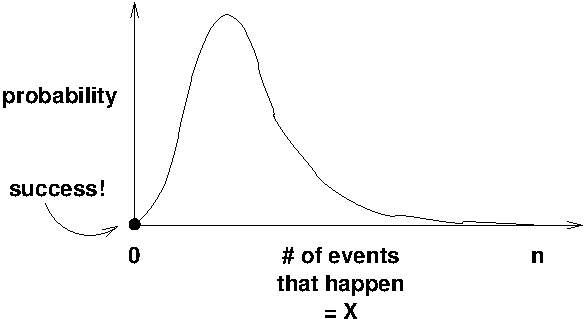
\includegraphics{pdf-x}
\end{center}
%
The spaceship flies successfully only if no critical parts fail; that
is, if $X = 0$.  In terms of the picture, the flight is successful
only at the absolute leftmost point of the distribution.  So in
analyzing the probability that the flight fails, we worked out general
bounds on the probability that we're \textit{not} at the tip of the
tail of the distribution:
%
\[
\underbrace{1 - e^{-\expect{X}}}_{
  \substack{\text{``Murphy's Law''} \\[0.5ex]
            \text{(if $E_1, \ldots E_n$ are independent)}}}
\leq \pr{E_1 \cup \ldots \cup E_n} \leq
\underbrace{\pr{E_1} + \ldots + \pr{E_n}}_{
  \substack{\text{Union Bound} \\[0.5ex]
            \text{(always holds)}}}
\]
%
In particular, Murphy's Law says that if many independent events are
expected to happen, then there's an extremely remote chance that none
of them will.  Thus, being out at the very tip of the tail is
\textit{extremely} weird.  In fact, we're next going to show than
being \textit{anywhere} in either tail of the distribution is pretty
unlikely.

\section{Chernoff Bounds}

MIT is admitting a new crop of students.  The Institvte has offered
admission to a few thousand applicants and carefully estimated the
probability that each will accept, based on his or her interests,
enthusiasm, and other likely offers.  This calculation indicates that
the expected number of new students is 1000, which is the ideal
number.  However, MIT must be wary of weird happenings.  If the new
class is too small, then expenses must be divided among fewer
students, forcing tuition up.  If the new class is too large, then
living conditions and classes will be crowded.  What is the
probability that MIT must cope with signficantly fewer or more
students?

Similar problems arise again and again in the analysis of computer
systems and algorithms.  The general theme is that there are many
events that \textit{can} occur, and we need to prove that the number
that actually \textit{do} occur is unlikely to be much greater or much
less than the expected number.  In terms of the probability density
function, we're trying to show that the tails are small:
%
\begin{center}
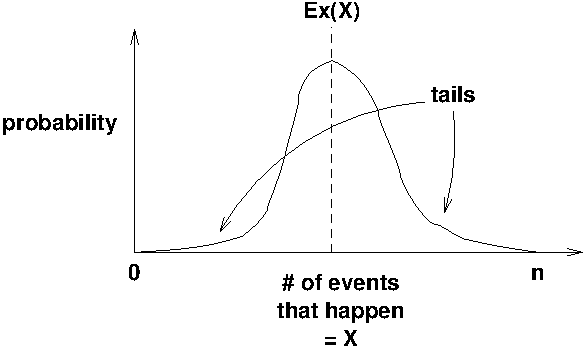
\includegraphics{pdf-x2}
\end{center}
%
If the events are mutually independent, then we can get quick results
to this effect from a powerful set of tools called \term{Chernoff
bounds}.

\begin{theorem}[Chernoff Bounds]
\label{th:chernoff}
Let $E_1, \ldots, E_n$ be a collection of mutually independent events,
and let $X$ be the number of these events that occur.  Then:
%
\begin{align*}
\pr{X \leq (1 - \delta) \expect{X}} & \leq e^{\textstyle -\delta^2 \expect{X} / 2}
    & \text{when $0 \leq \delta \leq 1$} \\[1ex]
\pr{X \geq (1 + \delta) \expect{X}} & \leq e^{\textstyle -\delta^2 \expect{X} / 3}
    & \text{when $0 \leq \delta \leq 1$} \\[1ex]
\pr{X \geq c \expect{X}} & \leq e^{\textstyle -(c \ln c - c + 1) \expect{X}}
    & \text{when $c \geq 1$}
\end{align*}
\end{theorem}

\noindent These are the supercharged Markov Inequalities that we
mentioned earlier.  The proof of this theorem is a bit intricate, so
let's first apply it to the admissions problem.

\subsection{MIT Admissions}

Let $E_k$ be the event that the $k$-th student accepts MIT's admission
offer.  Assume that all such events are mutually independent.  Let $X$
be the number of these events that occur; that is, $X$ is the size of
the incoming freshman class.  The all-knowing admissions office has
determined that $\expect{X} = 1000$.

We can upper bound the probability that the new class contains 900 or
fewer students using the first Chernoff inequality:
%
\begin{align*}
\pr{X \geq 900}
    & = \pr{X < \paren{1 - \frac{1}{10}} \expect{X}} \\
    & \leq e^{- (1/10)^2 \cdot 1000 / 2} \\
    & = e^{-5} \approx 0.0067
\end{align*}
%
On the other hand, we can upper bound the probability that 1200 or
more new students come to MIT using the second inequality:
%
\begin{align*}
\pr{X \geq 1200}
    & = \pr{X > \paren{1 + \frac{1}{5}} \expect{X}} \\
    & \leq e^{- (1/5)^2 \cdot 1000 / 3} \\
    & = e^{-40/3} \approx 0.0000016
\end{align*}
%
If we want to estimate the probability of a complete disaster---say,
3000 or more students accept---then we can no longer use the second
inequality; that holds only for deviations up to twice the
expectation.  We must use the third inequality instead.  (Actually,
the third Chernoff inequality always give an answer at least as good
as the second; however, the second is often more convenient.)
%
\begin{align*}
\pr{X \geq 3000}
    & = \pr{X > 3 \cdot \expect{X}} \\
    & \leq e^{-(3 \ln 3 - 3 + 1) \cdot 1000} \\
    & < e^{-1295}
\end{align*}
%
That's pretty unlikely!  

Like the Markov Inequality, a Chernoff bound may not yield the
strongest possible conclusion because it is supplied with very little
information about the random variable $X$.  However, Chernoff bounds
usually give \textit{good} results and they're very easy to apply.  So
Chernoff bounds should among the first tools you reach for when you
need to prove that weird things probably won't happen.

\subsection{Proving Chernoff Bounds}

Proving Chernoff bounds takes a good deal of work.  To demonstrate the
techniques involves, we'll prove the third inequality:
%
\[
\pr{X \geq c \expect{X}} \leq e^{\textstyle -(c \ln c - c + 1) \expect{X}}
    \qquad \text{when $c \geq 1$}
\]
%
The argument begins as follows:
%
\begin{align}
\pr{X \geq c \expect{X}}
  & = \pr{c^{X} \geq c^{\textstyle c \expect{X}}} \notag \\
  & \leq \frac{\expect{c^X}}{c^{\textstyle c \expect{X}}} \label{eqn:chernoffbase}
\end{align}
%
In the first step, we exponentiate both sides of the inequality with
base $c$.  The probability remains unchanged because both inequalities
describe the same event.  The second step uses Markov's Inequality.

These two steps illustrate the key idea behind Chernoff bounds.
Remember that Markov's Inequality upper bounds the probability that a
random variable deviates above the mean.  For some probability
distributions, Markov's Inequality gives a tight bound and for others
it doesn't.  Exponentiating before applying Markov's Inequality moves
us to the sweet spot of the Markov Inequality, ensuring that we get
good results.  This isn't the sort of trick you'd immediately think
up, but it works like a charm.

The next task is to find a convenient upper bound on the numerator
in~\eqref{eqn:chernoffbase}.  There are roughly three steps: break the
expression into little pieces, analyze each little piece, and then
assemble them back together again.  Let $I_1, \dots, I_n$ be
indicators for the events $E_1, \dots, E_n$.  In these terms, the
number of events that happen is:
%
\[
X = I_1 + \cdots + I_n
\]
%
We'll use this as our starting point:
%
\begin{align*}
\expect{c^X}
    & = \expect{c^{\textstyle \sum_{k=1}^n I_k}} \\
    & = \expect{\prod_{k=1}^n c^{I_k}} \\
    & = \prod_{k=1}^n \expect{c^{I_k}}
%
\intertext{The last step uses the fact that the indicators $I_k$ are
independent and the fact that functions of independent random
variables are themselves independent.  We've now decomposed the
original expression into a product of little pieces, each involving a
single indicator random variable.  The next step is to compute the
expected value of $c^{I_k}$ using the definition of expectation:}
%
    & = \prod_{k=1}^n \pr{E_k} \cdot c^1 +
                       (1 - \pr{E_k}) \cdot c^0 \\
    & = \prod_{k=1}^n 1 + (c-1) \pr{E_k} \\
    & \leq \prod_{k=1}^n e^{\textstyle (c-1) \pr{E_k}} \\
%
\intertext{On the last line we're using the inequality $1 + x \leq
e^x$.  Now we put all the pieces back together again:}
%
    & = e^{\textstyle \sum_{k=1}^n (c-1) \pr{E_k}} \\
    & = e^{\textstyle (c-1) \expect{X}}
\end{align*}
%
Plugging this upper bound into~\eqref{eqn:chernoffbase} gives:
%
\begin{align*}
\pr{X \geq c \expect{X}}
   & \leq \frac{e^{\textstyle (c-1) \expect{X}}}{c^{\textstyle c \expect{X}}} \\
   & = e^{\textstyle -(c \ln c - c + 1) \expect{X}} \\
\end{align*}
%
This is the third Chernoff inequality.  The second inequality follows
by setting $c = 1 + \delta$ and using an approximation based on the
Taylor series of the exponent.  The proof of the first inequality has
a similar structure, but differs in a few details.

A small corollary extends the usefulness of the Chernoff bounds in
further.  Sometimes we don't know $\expect{X}$ exactly, but we at least
know an upper bound.  Fortunately, the second and third Chernoff
inequalities still hold if we use this upper bound instead of the
exact value of $\expect{X}$.

\begin{corollary}
\label{cor:chernoff}
The second and third bounds in Theorem~\ref{th:chernoff} remain valid
when all instances of $\expect{X}$ are replaced by an upper bound on the
expectation of $X$.
\end{corollary}

The proof is a bunch of unenlightening algebra, which we'll omit.

\section{Hashing}

Suppose that we need to store credit histories for a great many
people.  We could create $n = 26^2$ bins labeled $AA, AB, AC, \ldots,
ZZ$.  Then we would store a person's record based on the first two
letters of their name.  For example, the record for ``Lee, Edmond''
would be stored in the bin labeled $LE$.  Then, when we needed to look
up Edmond's credit history, we would only need to search through the
records in bin $LE$, rather than all the records.

In computer science, this trick for rapidly storing and retrieving
records is called \textit{hashing}.  Each record consists of a
\textit{key} and \textit{value}.  A \textit{hash function} maps each
record's key to a bin.  In our example, the keys were names, the
values were credit histories, and the hash function mapped each name
to its first two letters.

The fear in hashing is that one bin somehow ends up with too many
records.  In that case, retrieving any record in the overloaded bin is
time-consuming, since there are so many to search through.  This sort
of imbalance is inevitable if the hash function is chosen poorly.  For
example, the hash function that maps each name to its first two
letters is actually a horribe choice because some two letter prefixes
are quite common ($LE$e, $LE$hman, $LE$ighton) and others extremely
uncommon ($QZ$, $VZ$, $RR$).

An ideal hash function would assign records to bins uniformly and
independently at random.  We can not achieve this goal in a rigorous
sense---there is really no randomization involved---but this is
still a decent practical model of a good hash function on typical
data.

So let's assume that $R$ records are hashed to $N$ bins uniformly and
independently at random.  Let's see what our various probability tools
say about the structure of the hash table.

\subsection{The First Collision}

When must there be a bin containing at least two records?

We can answer this question in two ways.  In an absolute sense, the
Pigeonhole Principle says that if there are $R > N$ records, then at
least one of the $N$ bins \textit{must} contains two or more records.

Alternatively, we could regard the records as people and the bins as
possible birthdays.  Then the Birthday Principle says that there is an
even chance that some bin contains two records when:
%
\[
R \approx \sqrt{(2 \ln 2) N}
\]
%
Thus, the first collision is likely to occur when the hash table still
contains very few records.  This can be frustrating.  For example, if
we create a hash table with a million bins, the probability that some
bin contains two records is $1/2$ when the table contains only about
1177 records!

\subsection{\emph{N} Records in \emph{N} Bins}

Suppose that the number of records in our hash table is equal to the
number of bins.  So, for example, we might be storing a million
records in a hash table with a million bins.  What does the table look
like?

Let's first consider a particular bin $B$.  Let $E_k$ be the event
that the $k$-record is hashed to bin $B$.  Since records are hashed
uniformly, $\pr{E_k} = 1/N$.  And these events are independent because
records are hashed to bins independently.

Now let $X$ be the number of these events that happen; that is, $X$ is
the number of records hashed to bin $B$.  The expected value of $X$ is
1 since:
%
\begin{align*}
\expect{X}
    & = \pr{E_1} + \ldots + \pr{E_N} \\
    & = N \cdot 1 / N \\
    & = 1
\end{align*}

We can use Murphy's Law to upper bound the probability that one or
more records are hashed to bin $B$:
%
\begin{align*}
\pr{E_1 \cup \ldots \cup E_N}
    & \geq 1 - e^{\expect{X}} \\
    & = 1 - 1 / e
\end{align*}
%
So $B$ is empty with probability at most $1 / e$.  Thus, the expected
number of empty bins in the whole table is at most $N / e \approx
0.367N$ and this bound is asymptotically tight.

We can upper bound the probability that bin $B$ gets more than $c$
records using the third Chernoff inequality.  Since $\expect{X} = 1$, this
has a simple form:
%
\begin{align*}
\pr{X \geq c} \leq e^{\textstyle -(c \ln c - c + 1)}
\end{align*}
%
How high must we set the threshold $c$ so that $\pr{X > c}$, the
probability that $c$ or more records are stored in bin $B$, is still
small?  Let's try $c = \ln N$:
%
\begin{align*}
\pr{X \geq \ln{N}}
    & \leq e^{\textstyle -(\ln N \ln \ln N - \ln N + 1)} \\
    & = \frac{1}{N^{\displaystyle \ln \ln N - 1 + 1 / \ln N}}
\end{align*}
%
The dominant term in the exponent is $\ln \ln N$, which tends to
infinity for large $N$.  So this probability goes to zero faster than
the inverse of any polynomial in $N$.  So, asymptotically, it is very
unlikely that any bin contains $\ln n$ or more records.

In fact, the probability that bin $B$ contains more than $c$ records
is still less than $1 / N^2$ when $c = e \ln N / \ln \ln N$.  (This
``log over log-log'' function comes up pretty often.  Say ``nice
function'' and let it sniff you.  Then give it a pat, and you'll be
friends for life.)  By the Union Bound, the probability that there
exists \textit{some} bin containing more than $c$ records is at most:
%
\begin{align*}
\pr{\text{some bin has } \geq \frac{e \ln N}{\ln \ln N}}
    &\leq \pr{\text{bin 1 does}} + \ldots + 
          \pr{\text{bin $N$ does}} \\
    & \leq N \cdot \frac{1}{N^2} \\
    & = \frac{1}{N}
\end{align*}
%
So, for example, if we put a million records into a million-bin hash
atable, then there is less than a 1-in-a-million chance that any bin
contains $15 > e \ln 10^6 / \ln \ln 10^6$ or more records.

\subsection{All Bins Full}

A final question: what is the expected number of records that we must
add to a hash table in order for every bin to contain at least 1
record?

This is a restatement of the Coupon Collector problem, which we
covered last time.  The solution is $R = N H_n \approx N \ln N$.  For
example, if the hash table contains $N = 1,000,000$ bins, then we must
add about $13.8$ million records to get at least one record in every
bin.

Unless something weird happens.
\end{editingnotes}
